\documentclass[a4paper]{article}
\usepackage{packages}
\usepackage{graphicx, float}
\usepackage{multicol}


\title{\LARGE VARIATIONAL MONTE CARLO METHOD APPLIED TO A SYSTEM OF INTERACTING BOSONS IN A ELLIPTICAL POTENTIAL \\ \vspace{5mm}  \large FYS4411 COURSE - COMPUTATIONAL PHYSICS II: QUANTUM MECHANICAL SYSTEMS \\ \large PROJECT 1 }
\author{\textsc{Emiliano Staffoli, Matteo Zortea, Alexander Ferraro }}
\date{\today}

\begin{document}

\pagenumbering{arabic}
\setcounter{page}{1}

\maketitle

\begin{abstract}
    put abstract here
\end{abstract}

\begin{multicols*}{2}
 \noindent

\section{INTRODUCTION}
\label{sec:introduction}
   A Bose-Einstein condensate is a state of matter that we can observe in a system of bosons confined and cooled down to temperatures close to the absolute zero. Since this physical concept was first proposed by Einstein and Bose \cite{einstein_original} in the 1920s, a lot of years have passed until the first experimental observation of this phenomenon, which was achieved by C. E. Wieman \& E. A. Cornell \cite{wieman} and W. Ketterle \cite{ketterle} only in 1995. Working independently, these two groups were able to observe a system of bosons constituted respectively by Rubidium atoms and Sodium atoms trapped at extremely low temperatures. 

Nowadays these systems are still intensively studied both from a experimental and theoretical perspective. In the former case, a BEC is produced in the laboratory exploiting laser cooling techniques and magnetic traps to confine the bosons \cite{lasercooling}. A theoretical analysis can instead be performed adopting a statistical approach, especially when the density of the system is sufficiently high to prevent from a proper description through the Gross-Pitaevskii equation \cite{gross}\cite{pita}. The problem can then be faced with the implementation of a Variational Monte Carlo (VMC) code: it allows to get pieces of information about a system using a statistical approach instead of trying to derive analytical solutions. Exploiting the concept of Markov chains \cite{markov} and algorithms based on pseudo-random numbers generation, we are allowed to explore all the possible states of a system and thus obtain numerical quantities related to it as averages over the possible configurations. The Monte Carlo method becomes particularly effective and time-saving when we have to deal with multidimensional integrals whose analytical evaluation would be impossible and the usage of traditional numerical methods would require a great effort. \\


In this project we are going to analyze the properties of a system constituted by $^{87}$Rb atoms through the implementation of a VMC code. We will consider a non-interacting hamiltonian and then switch to the interacting case, adopting for both the configurations a properly built trial wavefunction. The traps for the bosons will be described through a spherical or an elliptical potential. In our analysis we included also the search for the value of the variational parameter $\alpha$ corresponding to the minimum energy of the system. The VMC steps were performed exploiting different variants of the Metropolis algorithm. \cite{metropolis} \cite{hastings} (\textit{Add here missing parts about resampling methods and parallelization}).


\subsection{OVERVIEW OF THE WORKFLOW}
\textit{(We'll write this section at the end of the work, when everything will be defined)}
   
\section{THEORY AND MATHEMATICAL INSTRUMENTS}
\label{sec:theory}
    The treatment of complex many-body systems such as molecules or clusters represents a very demanding task. The introduction of some properly chosen approximations usually leads to a solution for the considered problem, the price to pay being a possible lack of accuracy in the obtained results. Extended systems illuminated by strong laser sources constitute a clear example: they are very complex to treat both computationally and theoretically and even the adoption of the so-called single active electron approximation is of any help in this context. Moreover, well known and established methods as the time-dependent Hartree-Fock or the time-dependent density functional theory suffer of a lack of accuracy when applied to the description of electron dynamics in such complex systems. Zanghellini et al. tried to provide for a new approach \cite{Zangellini_2003} to this kind of problems, formulating the so-called Multi-configuration time-dependent Hartree-Fock method for strong laser field problems. As the name suggests, this strategy still relies on the standard HF theory, but now the total wavefunction describing a system of fermions is expanded in a series of Slater determinants. Higher levels of accuracy can be reached as the number of terms $\eta$ in the expansion increases, finally reaching the exact solution for $\eta \rightarrow \infty$. 

At a later stage the validity of the approach was tested by applying it for the description of two systems, the first constituted by two electrons trapped in a harmonic oscillator potential, the second being represented by a He atom. Both the configurations were subject to a strong laser field. Procedures and results are reported in \cite{Zanghellini_2004}: here the attention is mainly focused on determining the number of Slater determinant that allows to reach a convergence with the numerically exact solution to the considered problems. On the contrary, we will limit our discussion to the case $\eta=1$, trying to reproduce the results for the 2-electrons systems only.

\subsection{PRELIMINARY TIME-INDEPENDENT TREATMENT}
The first part of the project was devoted to access the main properties of the system in its ground state. According to the content of the article, the following Hamiltonian was adopted
\begin{align}
\begin{split}
    H(x,y; t) =& -\frac{1}{2} \left( \frac{\partial^2}{\partial x^2} + \frac{\partial^2}{\partial y^2} \right) + \frac{1}{2} \Omega^2 (x^2 + y^2) + \\
    & + \frac{1}{\sqrt{(x-y)^2 + a^2}} \\
    =& \sum_{i=1}^2 h_i + v(x,y)
\end{split}  
\label{eq:hamiltonian_t_indep}
\end{align}
where $x$ and $y$ are the coordinates for the two electrons. The single-particle Hamiltonians are limited to a kinetic energy term and a harmonic oscillator potential, since at this stage the time dependence is still not included. The interaction between the electrons is represented by a smoothed Coulomb potential, where the shielding parameter $a$ has been inserted to avoid divergences. The values adopted in the article are $\Omega=0.25$, $\omega=8\Omega$ and $a=0.25$. \\

For this first stage of the treatment, the standard time-independent Hartree-Fock method was adopted. [bla bla bla, scriveremo qualcosa qui in base a dove mettiamo la derivazione].

\subsubsection{EXPECTATION VALUES}
The results in terms of total wavefunction $\Psi$ provided at the end of the iterative process were then used to access some important properties of the system in its ground state. In particular, the energy of the system can be achieved as
\begin{equation*}
    \mathbb{E}[H] =
\end{equation*}

% The Hamiltonian used for the description of the apparatus takes the following form (in atomic units)
% \begin{align}
% \begin{split}
%     H(x,y; t) =& -\frac{1}{2} \left( \frac{\partial^2}{\partial x^2} + \frac{\partial^2}{\partial y^2} \right) + \frac{1}{2} \Omega^2 (x^2 + y^2) + \\
%     &+ \frac{1}{\sqrt{(x-y)^2 + a^2}} + (x+y) \fakeeps_0 \sin (\omega t)
% \end{split}
% \label{eq:hamiltonian}
% \end{align}
% where $x$ and $y$ are the coordinates for the two electrons. The single-particle terms are constituted by an harmonic oscillator potential and a time-dependent sinusoidal contribution standing for the laser field illuminating the system. 

% \subsection{}



   
\section{METHODS}
\label{sec:methods}
    \subsection{VARIATIONAL MONTE CARLO}
While trying to access the properties of a system, one often has to deal with a coupled differential equations or with multidimensional integrals. In both these cases finding a solution is absolutely non trivial: an analytical expression could even not exist and using the traditional numeric methods can be very time consuming, especially for systems with a high number of degrees of freedom.

A possible alternative to face with these kind of problems is provided by the Variational Monte Carlo (VMC) method: this technique is based on a statistical approach and on the exploration of the possible configurations of a system through the generation of random numbers. At each step of a VMC simulation, a new proposal for a possible configuration of the system is created and properly implemented algorithms relying on pseudo-random numbers discriminate between the acceptance or rejection of such move. These algorithms are built to ensure that the states touched during the walk in the configurations' space reproduce the probability distribution for the system of being in a given state. After a sufficiently large number of steps (namely when this probability distribution is sufficiently well reconstructed) the quantities of interest for the considered system (e.g. energy) are provided as averages evaluated on the configurations explored during the simulation. 

The success of this technique is mainly due to its extreme versatility and to the fact that, as previously mentioned, it allows to avoid the direct treatment of integrals and differential equations. This methods reveals to be much effective in providing us with a result without needing to spend much effort in analytical or numerical evaluations. However, as it will be shown in the next sections, the results computed through this technique strongly depends on the knowledge of the function describing the probability for the system of being in a certain state. 


\subsection{LOCAL ENERGY}
One of the most relevant quantities in which we are interested for the characterization of our system is its ground state energy. The variational principle states that the expectation value of the hamiltonian evaluated on any wavefunction describing the system is an upper bound for the true ground state energy $E_0$. For our specific case, this reads 
\begin{align*}
    &E_0 \leq E [ \hat{H} ](\alpha) = \langle \Psi_T(\bm{R}, \alpha) \vert \hat{H} \vert \Psi_T(\bm{R}, \alpha) \rangle \\
    &= \frac{\int d\bm{R} \Psi_T^*(\bm{R}, \alpha) \hat{H} \Psi_T(\bm{R}, \alpha) }{\int d\bm{R} \Psi_T^*(\bm{R}, \alpha) \Psi_T(\bm{R}, \alpha)}
\end{align*}
where $\Psi_T(\bm{R},\alpha)$ is the trial wavefunction associated to the system and $\bm{R}$ is a collective variable containing all the coordinates of the particles in the problem. 

Our aim is then to find the value of $\alpha$ that minimized the integral reported above. A Variational Monte Carlo (VMC) simulation allows to face the problem of its evaluation. First one can define a probability density function $P(\bm{R}, \bm{\alpha})$ as
\begin{equation*}
    P(\bm{R}, \bm{\alpha}) = \frac{\vert \Psi_T (\bm{R}, \bm{\alpha}) \vert^2}{\int d\bm{R} \Psi_T^*(\bm{R}, \bm{\alpha}) \Psi_T(\bm{R}, \bm{\alpha}) }
\end{equation*}
which simply describes the probability to find the system in a given state in which particles' positions are described by the collective variable $\bm{R}$. Defining then the local energy $E_L (\bm{R}, \bm{\alpha})$ as 
\begin{equation}
    E_L(\bm{R}, \bm{\alpha}) = \frac{1}{\Psi_T(\bm{R}, \bm{\alpha})} \hat{H} \Psi_T(\bm{R}, \bm{\alpha})
    \label{local_energy}
\end{equation}
one can finally rewrite the expected energy value as
\begin{equation}
    E[\hat{H}](\alpha) = \int d\bm{R} P(\bm{R}, \bm{\alpha}) E_L(\bm{R}, \bm{\alpha})
    \label{energy_integral}
\end{equation}
At this point one can introduce a Monte Carlo estimator
\begin{equation}
    E[\hat{H}](\alpha) \simeq \frac{1}{N_s} \sum_{i=1}^{N_s} E_L(\bm{R}_i, \bm{\alpha})
    \label{montecarlo_estimator}
\end{equation}
where $N_s$ is the number of steps performed within a Monte Carlo simulation and $\bm{R}_1, \dots, \bm{R}_{N_s}$ are sets of positions sampled from the distribution $P(\bm{R}, \alpha)$. From a statistical point of view the law of large numbers guarantees that evaluating integral in Eq.\,\ref{energy_integral} is equivalent to evaluate the sum in Eq.\,\ref{montecarlo_estimator} if $N_s \to \infty$, but since this is obviously an unattainable condition one searches for a compromise between precision and computational cost. Better results in terms of both these aspects can be obtained with a previous knowledge of the analytical form of the local energy function. \\
For the system considered in this project it was possible to obtain an analytical expression for the energy of the system as a function $\alpha$ in the simple case of non-interacting particles in a spherical potential. This result will be adopted for comparisons with the estimates produced by the VMC code.
\begin{equation*}
    (instert-expression-here)
\end{equation*}



\subsubsection{ANALYTICAL FORM}
For the explicit calculations that lead to the results reported below, see \textit{Appendix} \ref{appendix:local_energy}. 

The analytic expression for the local energy in the case of a $D$-dimensional system of $N$ non-interacting particles subject to a spherical potential ($a=0$, $\beta=1$) results to be
\begin{equation*}
    E_L(\bm{R}, \alpha) = D N \alpha + \left( \frac{1}{2} - 2\alpha^2 \right) \sum_{j=1}^{N}  r_j^2
\end{equation*}

In the more complex case of interacting particles and elliptical potential, the result is
\begin{align*}
    &E_L(\bm{R}, \alpha) = \alpha (2 + \beta) N + \sum_i^N \bigg[ (x_i^2 + y_i^2)\left(\frac{1}{2} - 2\alpha^2 \right) + \\
    & + z_i^2\left( \frac{1}{2} \omega_z^2 - 2\alpha^2\beta^2 \right) \bigg] -  \frac{1}{2} \sum_i^N \sum_{j\neq i} \frac{a}{r_{ij}^2 (r_{ij} - a)} \times \\
    &\times \bigg\{ -4 \alpha \left( x_i, y_i, \beta z_i \right) \cdot \mathbf{r}_{ij} + 2 + \frac{a - 2r_{ij}}{ r_{ij} - a } + \\
    &+ \mathbf{r}_{ij} \cdot \sum_{m \neq i}   \frac{\mathbf{r}_{im}}{r_{im}} \frac{a}{r_{im} \left( r_{km} - a \right)} \bigg\} \bigg\}
\end{align*}





\subsubsection{NUMERICAL EVALUATION OF THE SECOND DERIVATIVE}
The local energy for the considered system can be estimated recurring to the numerical evaluation of the laplacian appearing in the Hamiltonian. In general, the second derivative of a function $f(x)$ in $x=x_0$ can be numerically approximated as
\begin{equation*}
    \frac{\partial^2 f (x_0)}{\partial x^2} \approx \frac{f(x_0 + h) + f(x_0-h) - 2 f(x_0)}{h^2}
\end{equation*}
where $h$ is a sufficiently small step. This method allows to avoid all the analytical calculations cited above, but provides less accurate results and a much greater computational effort. In fact, we can deduce that, according to Eq.\,\ref{hamiltonian} and Eq.\,\ref{local_energy}, to get the local energy for a $D$-dimensional system constituted by $N$ particles we need to evaluate the trial wavefunction $3ND$ times. The analytical approach described above is thus preferable, however this numerical alternative will be implemented for a comparison.


\subsection{METROPOLIS ALGORITHM}
As discussed in the previous section, by using a Monte Carlo approach our problem is reduced to simulate a random walk in the space of configurations for our system. Each new proposed state must be sampled from a given distribution: as a consequence, each possible configuration of the system should in principle be reachable within a sufficient number of steps. An algorithm that obeys this condition is called ergodic and this constitutes an essential requirement for a correct reconstruction of the PDF within a random walk in the configuration space. With the ergodic hypothesis we are trying to ensure that the results are not biased by the fact that the system remains always in the most probable configurations. 

A very simple and effective erogidic algorithm typically used with the Monte Carlo schematics for the generation of the new configuration at every step is the Metropolis one: it is based on the concept of Markov chain. We consider a generic PDF $P_i^{(n)}$ which provides the probability of finding the system in a state $i$ at time step $n$ (assuming to have discrete time). We can then introduce the so-called transition probability matrix $W(j \rightarrow i) = W_{ij}$ which instead gives the probability of a transition from state $i$ to state $j$ (in this context $P_i^{(n)}$ can be interpreted an element of a vector). For a Markov process it is true that
\begin{equation}
    P_i^{(n+1)} = \sum_{i} ( j \rightarrow i) P_j^{(n)} \iff \bm{P}^{(n+1)} = \bm{W} \bm{P}^{(n)}
    \label{markovchain}
\end{equation}
namely the probability of finding the system in state $i$ at time step $n+1$ depends only on the set of probabilities related to the previous instant. The following conditions must be also satisfied at every time step, due to the normalization of the probabilities
\begin{equation*}
    \sum_i P_i^{(n)} = \sum_j W_{ij} = 1
\end{equation*}
A Markov chain is said to be convergent if for sufficiently long times the temporal dependence contained in Eq.\,\ref{markovchain} disappears, in formulas
\begin{equation*}
     \bm{P}^{(n)} = \bm{W} \bm{P}^{(n)} \qquad \mbox{for } n \rightarrow \infty
\end{equation*}
It is possible to demonstrate that for a converging Markov chain the vector $\bm{P}^{(SS)} = \lim_{n\rightarrow \infty} \bm{P}^{(n)}$ representing the steady state (SS) for the chain coincides with the eigenvector of the transition probability matrix with eigenvalue $\lambda = 1$, which is also the highest eigenvalue for that matrix. The vector $\bm{P}^{(SS)}$ will then obey the following
\begin{equation}
    \bm{P}^{(SS)} = \bm{W} \bm{P}^{(SS)}
    \label{convergence_markov_chain}
\end{equation}
Assuming now the convergence of the Markov chain describing our system, we can go further in building the algorithm by modelling the elements of transition probability matrix as products between an acceptance probability and a transition probability
\begin{equation*}
    W(j\rightarrow i) = A(j\rightarrow i) T(j\rightarrow i)
\end{equation*}
This is completely legitimate, as in general the form of $\bm{W}$ is unknown. For both the matrices $A$ and $T$ the following condition applies
\begin{equation*}
    \sum_j A(j\rightarrow i) = \sum_j T(j\rightarrow i) = 1
\end{equation*}


The condition contained in Eq.\ref{convergence_markov_chain} becomes then
\begin{align*}
    P_i^{(SS)} &= \sum_j \left[ A(j\rightarrow i) T(j\rightarrow i) P_j^{(SS)} + (1 - A(i\rightarrow j)) T(i\rightarrow j) P_i^{(SS)} \right] \\
    &= \sum_j A(j\rightarrow i) T(j\rightarrow i) P_j^{(SS)} + P_i^{(SS)} \cancelto{1}{\sum_j T(i\rightarrow j)} - P_i^{(SS)} \sum_j A(i\rightarrow j) T(i\rightarrow j)  \\
    &= P_i^{(SS)} + \sum_j \left[ A(j\rightarrow i) T(j\rightarrow i) P_j^{(SS)} -  A(i\rightarrow j) T(i\rightarrow j) P_i^{(SS)}  \right]
\end{align*}
In principle imposing that the sum is null does not prevent cyclic solutions for Eq.\,\ref{convergence_markov_chain}, and thus a stronger statement is required. Setting each term of the sum to be null guarantees the validity of the equation and we obtain the detailed balance condition
\begin{equation}
    \frac{A(j\rightarrow i)}{A(i\rightarrow j)} =  \frac{ T(i\rightarrow j) P_i^{(SS)}}{T(j\rightarrow i) P_j^{(SS)}}
    \label{metropolis_ratio}
\end{equation}
This is the driving equation for the Metropolis algorithm that we are going to use for the VMC code implemented in this project. The algorithm is built in such a way that, starting from a state $j$ it will propose a transition to a state $i$ with a given probability $T(j\rightarrow i)$, but then the move will indeed be accepted with a probability $A(j\rightarrow i)$. This last function is modelled by the Metropolis algorithm as
\begin{equation*}
    A(j\rightarrow i ) = \text{min} \bigg\{ 1, \frac{T(i \rightarrow j) P_i^{(SS)}}{T(j\rightarrow i) P_j^{(SS)}} \bigg\}
\end{equation*}
With this we impose that the system will surely move to a new proposed state if the ratio of Eq.\,\ref{metropolis_ratio} is greater than 1, otherwise the move will be accepted only if a generated random number is smaller than the ratio itself. This choice for the acceptance probability ensures that every possible state of the system can in principle be explored within a sufficiently long amount of steps and thus the ergodic hypothesis is preserved. Moreover, since we are considering the ratio of two PDFs $P_i$ and $P_j$, any problem due to the evaluation of multidimensional integrals totally disappears. 

Possible models for the transition probability matrix $T(j\rightarrow i)$ and for the generation of the new configurations for the system are discussed below.



\subsection{Brute-force Metropolis algorithm}
A suitable choice for the transition probability matrix consists in imposing a symmetry condition, namely $T( i\rightarrow j) = T(j \rightarrow i)$. For each step of the VMC simulation the algorithm acts as follows
\begin{itemize}
    \item considering a randomly selected particle, each  component $k = \{x,\,y,\,z\}$ of its position vector is modified according to
    \begin{equation*}
        (\bm{r}')_k = (\bm{r})_k + \Delta x \ast \eta
    \end{equation*}
    where $\eta \in (-0.5, 0.5)$ is a random number generated from a uniform distribution and $\Delta x$ is a step length chosen by the user;
    \item this move gets actually accepted if $\eta' < A(j\rightarrow i)$, with $\eta' \in (0,1)$ is another random number generated from a uniform distribution and
    \begin{equation*}
        A(j \rightarrow i) = \text{min} \bigg\{ 1, \frac{P_i}{P_j} \bigg\}
    \end{equation*}
\end{itemize}
We notice that in order to let the algorithm work correctly it is necessary to choose a proper step $\Delta x$: a too short value would imply that a higher number of Monte Carlo step is needed to reach the convergence of the Markov chain and to explore all the configurations of the system. On the contrary, a too large step would produce a very low fraction of accepted moves during the computation, especially if the wavefunction is particularly peaked in a specific region of the space. Generally the step length used for the brute-force Metropolis algorithm is set by a comparison with the typical length which characterises the system. For our specific case, starting from the hamiltonian of Eq.\,\ref{hamiltonian} it is possible to demonstrate (see \textit{Appendix B}) that this typical length unit corresponds to 
\begin{equation*}
    \Delta x = \sqrt{\frac{m \omega}{\hbar}}
\end{equation*}
In any case, as a rule of thumb we could state that a properly chosen step length should provide a $50\%$ acceptance ratio. 






\subsection{Importance Sampling}
In the brute-force Metropolis algorithm the generation of the new possible state for the system is entirely based on a uniformly distributed random variable and the information provided by the PDF for the system comes to play only at the moment of the evaluation of the acceptance probability. On the contrary, one could think of exploiting the PDF already at the moment of the generation of the proposed transition so that the system is more likely to go towards high-probability configurations. This would lead to an increased acceptance ratio, meaning a more efficient simulation. This is the core of the Importance sampling method in the context of Metropolis algorithm.

The idea just illustrated can be implemented starting from the Fokker-Plank equation, which describes the behaviour of a time-dependent PDF $P(\bm{r}, t)$ associated to a diffusive process characterized by a diffusion coefficient $D$. The equation reads
\begin{equation*}
    \frac{\partial P(\bm{r}, t)}{\partial t} = D \sum_i \frac{\partial}{\partial \bm{r}_i} \left( \frac{\partial}{\partial \bm{r}_i} - \bm{F}_i \right) P(\bm{r}, t)
\end{equation*}
where $i$ is an index running on the components $\{x,\,y,\,z\}$. The function $\bm{F}$ represent the aforementioned drift force term that we want to introduce in order to guide the system towards high-probability regions of the configurations space. The form of this drift force can be deduced by requiring that after the thermalization of the system (namely after a sufficiently long simulation time) the PDF will converge to a time-independent steady-state solution $P(\bm{r})$. It is possible to proof that this condition is reached if $\bm{F}$ assumes the following form
\begin{equation*}
    \bm{F}(\bm{r}) = \frac{1}{P(\bm{r})} \nabla P(\bm{r})
\end{equation*}
The fundamental role played by this drift force in the problem becomes clearer when we consider the Langevin equation, which describes the diffusive motion of a particle under the action of a drift force $\bm{F}(x(t))$ and a random contribution $\bm{\eta}$ 
\begin{equation*}
    \frac{\partial \bm{r}(t)}{\partial t} = D \bm{F}(\bm{r}(t)) + \bm{\eta}  
\end{equation*}
By solving this differential equation assuming a discrete time step $\delta t$, we get a new algorithm for the generation of the proposed move for a randomly chosen particle, namely
\begin{equation*}
    \bm{r}' = \bm{r} + D \bm{F}(\bm{r}) \delta t + \xi \sqrt{\delta t}
\end{equation*}
where $\xi$ is a gaussian random variable with null mean value and unitary standard deviation. Here we can clearly appreciate the effect of the drift force: in fact it will introduce a tendency for the particles to generate high-probability configurations by pushing them towards regions where the PDF is flat and high-valued. A single move is then more likely to be accepted. We notice that even with this new way of generating the propose for the new position of the particles, the erogdicity of the algorithm is still preserved, since every state can possibly be reached within a sufficiently high number of steps. 

Finally, by solving the Fokker-Plank equation it is possible to derive an expression form for the transition probability appearing in Eq.\,\ref{metropolis_ratio}, which results to be in the form of the Green's function, namely
\begin{equation*}
    G(\bm{r}', \bm{r}, t) = \frac{1}{\left (4 \pi D \delta t\right)^{3N/2}} \exp \left[ - \frac{ \left( \bm{r}' - \bm{r} - D\delta t \bm{F}(t)\right)^2}{4D\delta t}  \right]
\end{equation*}

The importance sampling algorithm will then act as follows:
\begin{itemize}
    \item considering a randomly selected particle, each  component $k = \{x,\,y,\,z\}$ of its position vector is modified according to
    \begin{equation*}
        (\bm{r}')_k = (\bm{r})_k + D \delta t \bm{F}_k + \xi \sqrt{\delta t}
    \end{equation*}
    where $\xi$ is a gaussian random variable with $\mu = 0$ and $\sigma=1$, while $\Delta t$ is the time step chosen by the user;
    \item this move gets actually accepted if $\eta < A(j\rightarrow i)$, with $\eta \in (0,1)$ is a random number generated from a uniform distribution and
    \begin{equation*}
        A(j \rightarrow i) = \text{min} \bigg\{ 1, \frac{P(\bm{r}')}{P(\bm{r})} \frac{G(\bm{r}', \bm{r}, \delta t)}{G(\bm{r}, \bm{r}', \delta t)} \bigg\}
    \end{equation*}
\end{itemize}




    
\section{CODE STRUCTURE}
\label{sec:code}
\begin{figure}[H]
    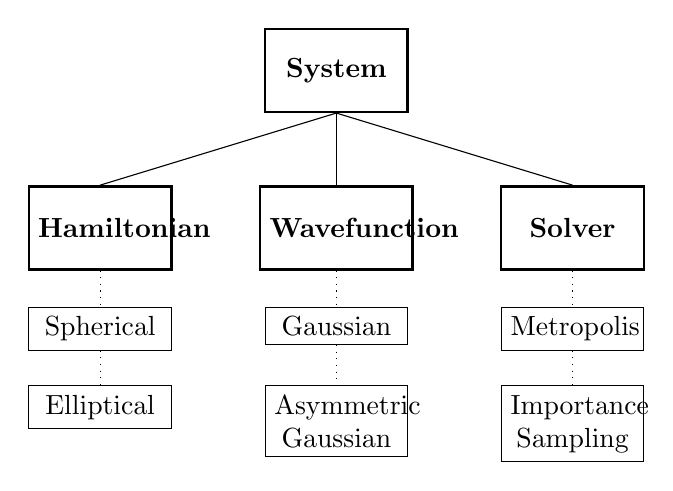
\begin{tikzpicture}
        
        \node (system) [draw, line width=0.3mm, text width=0.13\textwidth, minimum height=30pt, text centered] at (0,2) {\bfseries System};
        
        \node (wavefunction) [draw, line width=0.3mm, text width=0.14\textwidth, minimum height=30pt, text centered] at (0,0) {\bfseries Wavefunction};
        \node (gauss) [draw, anchor=north, text width=0.13\textwidth, text centered] at (0, -1) {Gaussian};
        \node (asymmgauss) [draw, anchor=north, text width=0.13\textwidth, text centered] at (0, -2) {Asymmetric \\ Gaussian};
        
        \node (solver) [draw, line width=0.3mm, text width=0.13\textwidth, minimum height=30pt, text centered] at (3,0) {\bfseries Solver};
        \node (metropolis) [draw, anchor=north, text width=0.13\textwidth, text centered] at (3, -1) {Metropolis};
        \node (importance) [draw, anchor=north, text width=0.13\textwidth, text centered] at (3, -2) {Importance \\ Sampling};
        
        \node (hamiltonian) [draw, line width=0.3mm, text width=0.13\textwidth, minimum height=30pt, text centered] at (-3,0) {\bfseries Hamiltonian};
        \node (spherical) [draw, anchor=north, text width=0.13\textwidth, text centered] at (-3, -1) {Spherical};
        \node (elliptical) [draw, anchor=north, text width=0.13\textwidth, text centered] at (-3, -2) {Elliptical};
        
        \draw (system.south) -- (wavefunction.north);
        \draw (system.south) -- (hamiltonian.north);
        \draw (system.south) -- (solver.north);
        
        \draw [dotted] (hamiltonian.south) -- (spherical.north);
        \draw [dotted] (spherical.south) -- (elliptical.north);
        \draw [dotted] (wavefunction.south) -- (gauss.north);
        \draw [dotted] (gauss.south) -- (asymmgauss.north);
        \draw [dotted] (solver.south) -- (metropolis.north);
        \draw [dotted] (metropolis.south) -- (importance.north);
    \end{tikzpicture}
    \caption{Classes diagram and hierarchy. Elliptical and spherical are Hamiltonian's subclasses, Gaussian and AsymmetricGaussian are Wavefunction's sublclasses, Metropolis and ImportanceSampling are Solver's sublasses.}
    \label{diag:classes_diagram}
\end{figure}
We chose C\texttt{++} as the main programming language to implement the aforementioned methods for this project. This allowed us to keep a good compromise between computational speed and abstraction. The algorithm has been fully object oriented making the code modular, in the sense one can in principle reuse the code for other purposes by only replacing some pieces and keeping the general structure. All the implemented classes can be classified into three categories:
\begin{itemize}
    \item \emph{System}: contains information on the system as a whole like the collection of particle and provides a reference point for communication between the other classes;
    \item \emph{Solvers} which provides different tools to evaluate the ground state of the chosen hamiltonian with the chosen wavefunction on different complexity levels, depending on the needs;
    \item \emph{Wavefunctions};
    \item \emph{Hamiltonians}.
\end{itemize}
The code has been documented via Doxygen and the documentation, together with the code itself, can be found at the GitHub link provided at the end of the report, hence hereby we discuss only some of the peculiar points of the implementation.
\subsection*{Wavefunction evaluation in the non-interacting case}
In the non-interacting case we exploited the relatively simple form of the local energy and the wavefunction to evaluate the Monte Carlo cycles in a more efficient way. In particular, at each cycle, we generated a proposal move for one particle only and evaluated the new wavefunction and the new local energy just by adjusting the values taken in the previous cycle since the dependence of each particle enters in the formulae only trough multiplicative factors or summation terms. To be more precise, if the wavefunction at the step $k$ of the algorithm is
$$\psi^{k} \equiv \psi(\bm{r}(t_k)) = \prod_{i=1}^{N} g(\alpha, \bm{r}_i(t_k)) \equiv \prod_{i=1}^N g_i^{(k)}$$
then, if at the step $k+1$ we modify the position of the particle $n$, the wavefunction becomes
$$\psi^{k+1} \ = \ g_n^{(k+1)} \, \prod_{\substack{i=1\\ i \neq n}} g_i^{k}$$
The relation for the local energy follows in a similar way.
\subsection*{Relative position in the interacting case}
The interacting case leads to way more complicated expressions and a clever way to evaluate the necessary quantities as done with the non-interacting case is not so immediate. However we noticed the repetitive demand for the same quantities, like the relative positions and relative distances between particles, in different expression, hence we stored those values in proper matrices avoiding repetitive re-evaluations of those high time-demanding operations. The $ij$-th element of the distance matrix $D_{ij}$ is the distance between the particle $i$ and particle $j$: here one can note that this matrix is symmetrical, hence only one half of the off-diagonal values must be computed. In a similar way the $ij$-th element of the relative position matrix $R_{ij} = \bm{r}_i - \bm{r}_j$ is the relative position, in cartesian coordinates, of the particles $i$ with respecto to the particle $j$: this matrix is antisymmetrical, hence, also in this case, only half of the off-diagonal element can be computed. The matrices are built and initialised at the beginning of the program, and after one particle is moved, only the corresponding rows and columns in the matrices are updated.
\subsubsection*{Code parallelization}
Various part of the code have been parallelized via OpenMP. \\
\dots Spiegare cosa e quali \dots 


\section{RESULTS}
\label{sec:results}
The analysis of the results produced by our code passed through a series of intermediate and progressive steps, continuously checking the outcomes obtained via the simulation with the analytical formulas, fortunately available for the non-interacting case. We will now proceed with the presentation of the results derived within the context of our project, enlightening the features of any performed simulation and the methods to validate the solidity and efficiency of the code. First we will focus on the runs carried out in non-interacting case both with the brute-force Metropolis algorithm and the importance sampling, proceeding then towards a more detailed statistical analysis through the blocking method. Then the interaction between particles will be introduced, together with the gradient descent method for the research of the $\alpha$ which minimizes the energy and then concluding with the one-body density evaluation.


\subsection{NON-INTERACTING SYMMETRICAL CASE}
\subsubsection{BRUTE-FORCE METROPOLIS ALGORITHM}
At first we chose a spherical potential trap with a simple gaussian trial wavefunction, these obtained by setting $a=0$ and $\beta=1$ into Eq.\,\ref{wavefunctions} and adopting the potential described in Eq.\,\ref{spherical_pot}. In order to obtain a numerical estimation of the ground state energy of the system we first adopted the so called Brute-Force Metropolis algorithm, previously introduced. We performed different simulations varying many parameters of the system and before each of these runs the system was submitted to $10^5$ thermalization steps. This choice has been preserved for each simulation presented from now on in the report. In principle we could have reduced the number of thermalization steps for the most simple configurations, involving for example 1 particle in a 1-dimensional system. However, since the most time-demanding operation is the evaluation of the local energy (not performed for the thermalization steps), the computational time for the initialization is considerably low, even with such an amount of steps and a large number of particles. We notice also that with the highest number of particles adopted for the system ($N=500$), within a $10^5$-steps thermalization process each of them will on average be moved 200 times, which we retained sufficient for the considered Markov chain to converge to the stationary PDF. \\

Table \ref{tab:tab_x_metropolis_analytical} reports the results of the analysis of the system's dependence on the number of particles and dimension. The value of $\alpha$ was kept fixed at $\alpha = 0.5$. The corresponding results obtained using the numerical method to evaluate the second derivative are reported in Table \ref{tab:tab_x_metropolis_numerical}. One can immediately notice a reduction in the precision and a significant increase in the simulation time with the numerical approach, hence leaving the only purpose of this second method to perform preliminary tests and qualitative studies. Proceeding, Figure \ref{fig:varying_alpha_noninteract_metropolis}, shows the value of the ground state energy of the system as a function of the parameter $\alpha$ for a particular configuration of the simulation settings, that is $N=10$ particles, 3 dimensions, $2^{21}$ steps and Metropolis step-size $r_{step} = 1.0$. One can immediately notice that the function is convex, which guarantees the existence of one unique minimum point, in accordance to what discussed in the context of the gradient descent method. In this simple case, the convexity of the energy curve as a function of $\alpha$ was expected, as it can be derived from the analytical form available in Eq.\,\ref{energy_analitical}. Some selected results for different $\alpha$ values are reported also in Table \ref{tab:varying_alpha_noninteracting}, referring to simulations performed again for a $3D$ system with $N=10$ particles and $N_{steps}=2^{21}$. This table contains also a comparison between the variance calculated as $\sigma^2_E = (\langle E_L^2 \rangle - \langle E_L \rangle^2)/N_{steps}$ and the variance calculated via the blocking method as explained in Section \ref{sec:blocking_method}.

\begin{table}[H]
    \centering
    \begin{tabular}{cccccc}
    \toprule
    $N_{part}$ & $N_{dim}$ & $\langle E_L \rangle$ & $\sigma_E$ & $t_{CPU}\;[s]$ & acc.ratio \\
    \midrule
    1 & 1 & 0.50000 & 0.00000 & 0.250 & 0.7293 \\
    1 & 2 & 1.0000 & 0.00000 & 0.277 & 0.5958 \\
    1 & 3 & 1.5000 & 0.00000 & 0.293 & 0.5053 \\
    \midrule
    10 & 1 & 5.0000 & 0.00000 & 0.397 & 0.7290 \\
    10 & 2 & 10.000 & 0.00000 & 0.426 & 0.5956 \\
    10 & 3 & 15.000 & 0.00000 & 0.453 & 0.5047 \\
    \midrule
    100 & 1 & 50.000 & 0.00000 & 1.967 & 0.7287 \\
    100 & 2 & 100.00 & 0.00000 & 2.084 & 0.5950 \\
    100 & 3 & 150.00 & 0.00000 & 2.388 & 0.5043 \\
    \midrule
    500 & 1 & 250.00 & 0.00000 & 20.695 & 0.7293 \\
    500 & 2 & 500.00 & 0.00000 & 22.008 & 0.5961 \\
    500 & 3 & 750.00 & 0.00000 & 21.776 & 0.5051 \\
    \bottomrule
    \end{tabular}
    \caption{The table reports the results of the simulations performed in the non-interacting case using a simple gaussian trial wavefunction and a brute-force Metropolis sampling method with $N_{therm}=10^5$, $N_{steps}=2^{21}$, step-size set to $r_{step}=1.0$ and constant value for $\alpha=0.5$. The local energy is evaluated exploiting the analytical formula and $\sigma_E$ is the error on $\langle E_L \rangle$ estimated from the standard deviation of of the $E_L$ samples generated during the run. }
    \label{tab:tab_x_metropolis_analytical}
\end{table}

\begin{table}[H]
    \centering
    \begin{tabular}{cccccc}
    \toprule
    $N_{part}$ & $N_{dim}$ & $\langle E_L \rangle $ & $\sigma_E$ & $t_{CPU}$ & acc.ratio \\
    \midrule
    1 & 1 & 0.5000000000 & 7\e-10 & 0.497 & 0.7290 \\
    1 & 2 & 1.000000000 & 1\e-9 & 0.631 & 0.5949 \\
    1 & 3 & 1.500000000 & 2\e-9 & 0.799 & 0.5050 \\
    \midrule
    10 & 1 & 5.000000006 & 2\e-9 & 2.217 & 0.7296 \\
    10 & 2 & 10.000000000 & 3\e-9 & 2.975 & 0.5960 \\
    10 & 3 & 15.000000010 & 5\e-9 & 4.035 & 0.5051 \\
    \midrule
    100 & 1 & 49.999999913 & 7\e-9 & 20.71 & 0.7287 \\
    100 & 2 & 99.99999991 & 1\e-8 & 28.49 & 0.5957\\
    100 & 3 & 149.99999965 & 2\e-8 & 37.02 & 0.5057 \\
    \midrule
    500 & 1 & 250.99999950 & 1\e-8 & 237.05 & 0.7298 \\
    500 & 2 & 500.00000067 & 2\e-8 & 347.24 & 0.5952 \\
    500 & 3 & 749.99999921 & 3\e-8 & 413.98 & 0.5045 \\
    \bottomrule
    \end{tabular}
    \caption{The table reports the results of the simulations in the non-interacting case using a simple gaussian trial wavefunction and a brute-force Metropolis sampling method with $N_{therm}=10^5$,  $N_{steps}=2^{21}$, step-size set to $r_{step}=1.0$ and constant value for $\alpha=0.5$. The local energy is evaluated exploiting the numerical second derivative and $\sigma_E$ is the error on $\langle E_L \rangle$ estimated from the standard deviation of the $E_L$ samples generated during the run. }
    \label{tab:tab_x_metropolis_numerical}
\end{table}

\begin{figure}[H]
    \centering
    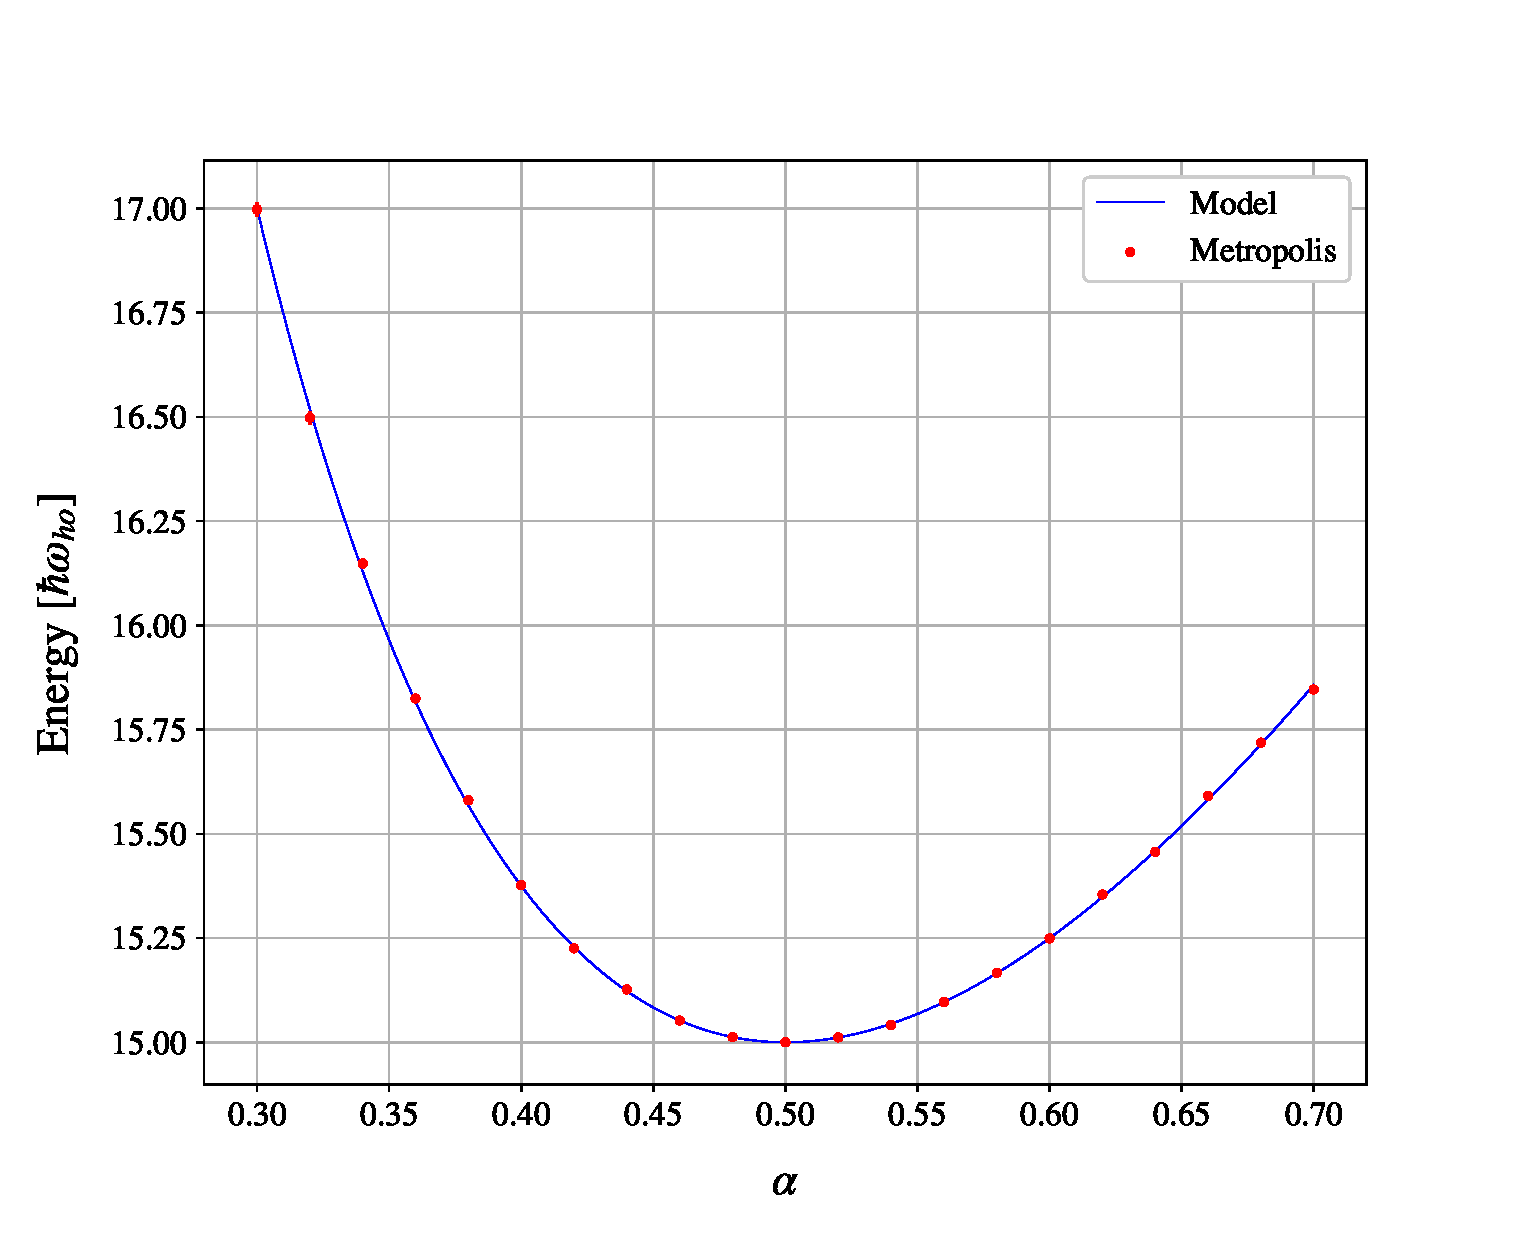
\includegraphics[scale=0.37]{images/varying_alpha_noninteract_metropolis.eps}
    \caption{The figure reports the energy estimates as a function of $\alpha$ generated by various VMC simulations exploiting the brute-force Metropolis algorithm with $N_{therm}=10^5$, $N_{steps}=2^{21}$ and $r_{step}=1.0$. The curve is referred to a $3D$ system with $N=10$ non-interacting particles. For some of the points the errorbar is too small to be seen. }
    \label{fig:varying_alpha_noninteract_metropolis}
\end{figure}


\subsubsection{IMPORTANCE SAMPLING}
The immediate improvement of this simple model was the inclusion of the importance sampling. This allowed us to bias the random walk in the configuration space according to the probability distribution, leading thus to higher number of accepted steps in the Monte Carlo run. As for the Brute Force Metropolis, results for fixed $\alpha=0.5$ obtained with the analytical and numerical evaluation of the local energy are reported respectively in Table \ref{tab:tab_x_importance_analytical} and Table \ref{tab:tab_x_importance_numerical}. The estimated energy as a function of $\alpha$ for a $3D$ system populated by 10 particles is reported in Figure \ref{fig:varying_alpha_noninteract_importance} with some selected results in Table \ref{tab:varying_alpha_noninteracting}. All the simulations cited above have been carried out with $2^{21}$ Monte Carlo steps and $\delta t = 0.1$. 


\begin{table}[H]
    \centering
    \begin{tabular}{cccccc}
    \toprule
    $N_{part}$ & $N_{dim}$ & $\langle E_L \rangle$ & $\sigma_E$ & $t_{CPU}$ & acc. ratio \\
    \midrule
    1 & 1 & 0.50000 & 0.00000 & 0.373 & 0.9928  \\
    1 & 2 & 1.0000 & 0.00000 & 0.385 & 0.98877 \\
    1 & 3 & 1.5000 & 0.00000 & 0.432 & 0.9857 \\
    \midrule
    10 & 1 & 5.0000 & 0.00000 & 0.714 & 0.9929 \\
    10 & 2 & 10.000 & 0.00000 & 0.792 & 0.9889 \\
    10 & 3 & 15.000 & 0.00000 & 0.793 &  0.9858 \\
    \midrule
    100 & 1 & 50.000 & 0.00000 & 4.197 & 0.9929 \\
    100 & 2 & 100.00 & 0.00000 & 4.378 & 0.9887 \\
    100 & 3 & 150.00 & 0.00000 &  4.339 & 0.9856 \\
    \midrule
    500 & 1 & 250.00 & 0.00000 & 36.624 & 0.9929 \\
    500 & 2 & 500.00 & 0.00000 & 39.380 & 0.9888 \\
    500 & 3 & 750.00 & 0.00000 & 39.965 & 0.9858 \\
    \bottomrule
    \end{tabular}
    \caption{The table reports the results of the simulations in the non-interacting case using a simple gaussian trial wavefunction and the importance sampling method with $N_{therm}=10^5$, $N_{steps}=2^{21}$, $\delta t = 0.1$ and constant value for $\alpha=0.5$. The local energy is evaluated exploiting the analytical formula and $\sigma_E$ is the error on $\langle E_L \rangle$ estimated from the standard deviation of the $E_L$ samples generated during the run. }
    \label{tab:tab_x_importance_analytical}
\end{table}

\begin{table}[H]
    \centering
    \begin{tabular}{cccccc}
    \toprule
    $N_{part}$ & $N_{dim}$ & $\langle E_L \rangle$ & $\sigma_E$ & $t_{CPU}$ & acc.ratio \\
    \midrule
    1 & 1 & 0.5000000027 & 7\e-10 & 0.761 & 0.9928 \\
    1 & 2 & 1.000000000 & 1\e-9 & 0.961 & 0.9888 \\
    1 & 3 & 1.500000004 & 2\e-9 &  1.332 & 0.9856\\
    \midrule
    10 & 1 & 4.999999937 & 2\e-9 & 3.311 & 0.9928 \\
    10 & 2 & 10.000000039 & 3\e-9 & 5.772 & 0.9887 \\
    10 & 3 & 15.000000053 & 5\e-9 & 8.097 & 0.9857 \\
    \midrule
    100 & 1 & 49.999999990 & 7\e-9 & 31.444 & 0.9929 \\
    100 & 2 & 99.99999966 & 1\e-8 & 55.850 & 0.9888 \\
    100 & 3 & 150.00000048 & 2\e-8 & 85.201 & 0.9857 \\
    \midrule
    500 & 1 & 250.00000078 & 1\e-8 & 323.70 & 0.9927 \\
    500 & 2 & 500.00000208 & 2\e-8 & 540.58 & 0.9886 \\
    500 & 3 & 749.99999858 & 3\e-8 & 877.82 & 0.9859 \\
    \bottomrule
    \end{tabular}
    \caption{The table reports the results of the simulations in the non-interacting case using a simple gaussian trial wavefunction and the importance sampling method with $N_{therm}=10^5$, $N_{steps}=2^{21}$, $\delta t = 0.1$ and constant value for $\alpha=0.5$. The local energy is evaluated exploiting the numerical evaluation of the second derivative and $\sigma_E$ is the error on $\langle E_L \rangle$ estimated from the standard deviation of the $E_L$ samples generated during the run.  }
    \label{tab:tab_x_importance_numerical}
\end{table}

\begin{figure}[H]
    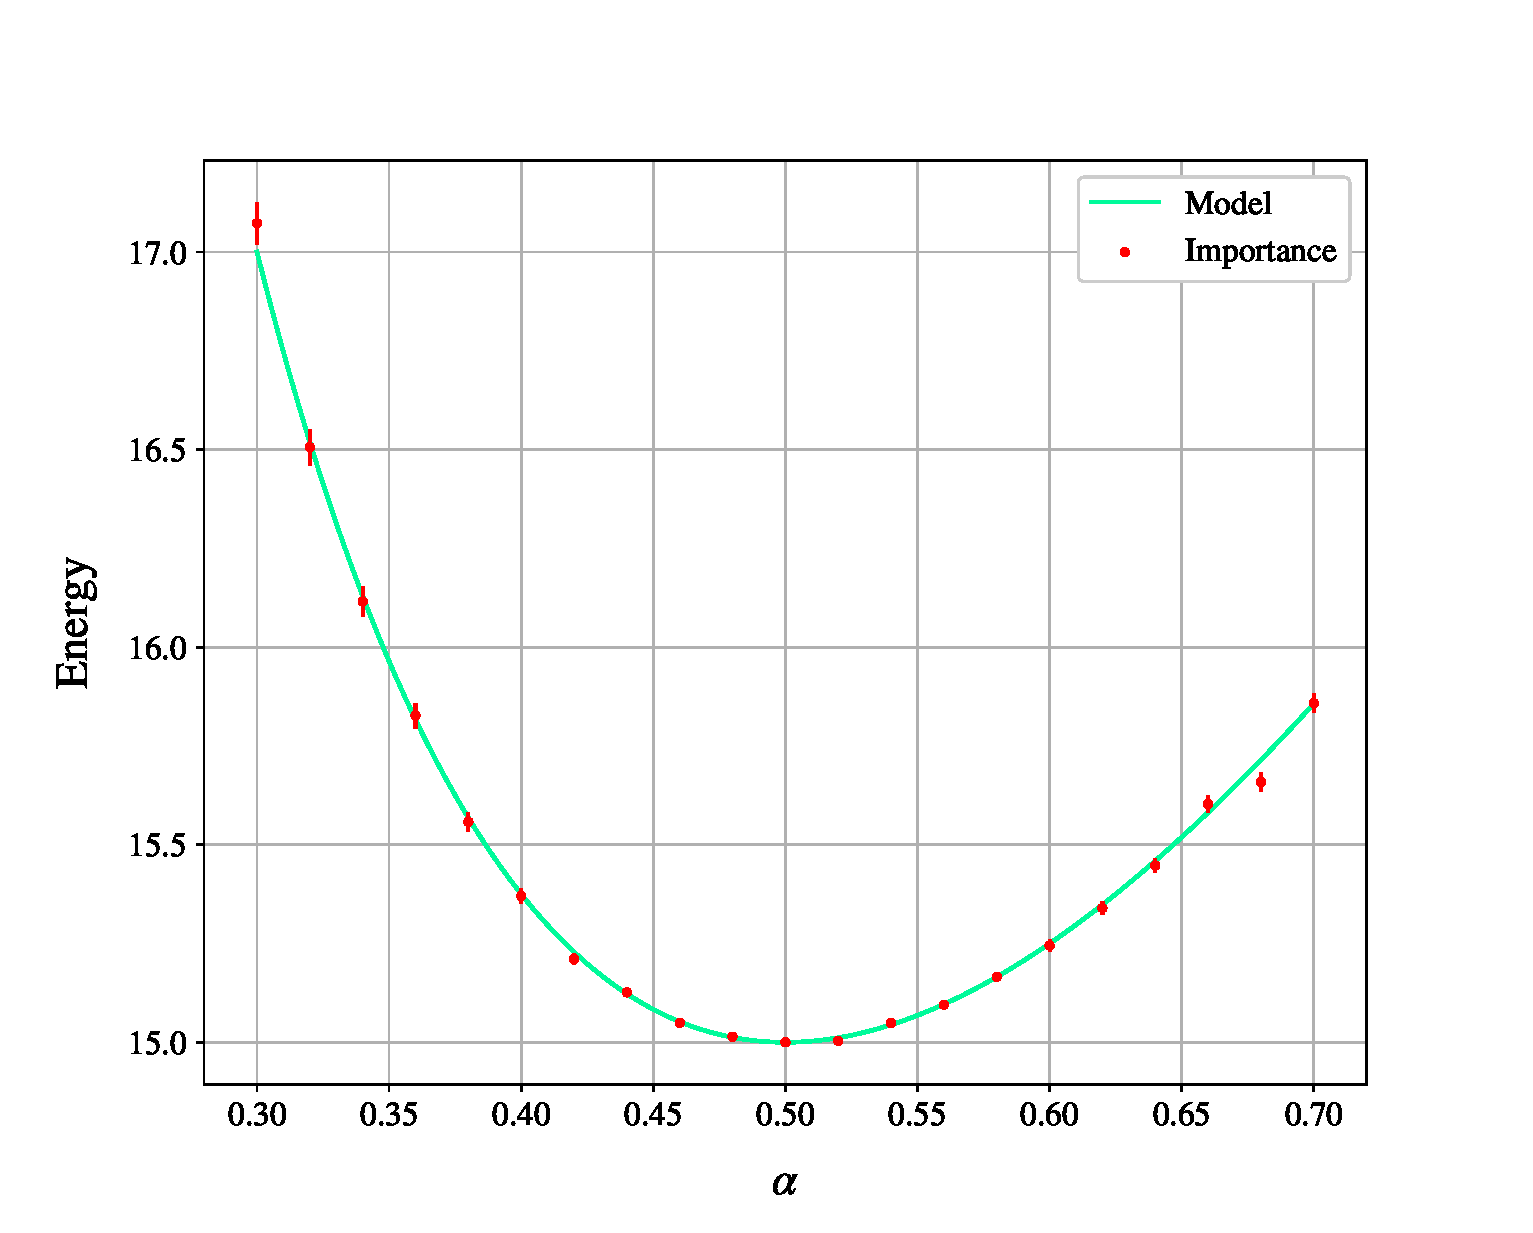
\includegraphics[scale=0.37]{images/varying_alpha_noninteract_importance.eps}
    \caption{The figure reports the energy estimates as a function of $\alpha$ generated by various VMC simulations exploiting the importance sampling with $N_{therm}=10^5$, $N_{steps}=2^{21}$, $\delta t = 0.1$. The curve is referred to a $3D$ system with $N=10$ non-interacting particles. For some of the points the errorbar is too small to be seen. }
    \label{fig:varying_alpha_noninteract_importance}
\end{figure}


\begin{table}[H]
    \centering
    \begin{tabular}{ccccc}
    \toprule
        \multicolumn{5}{c}{Metropolis} \\
        \midrule
        $\alpha$ & $\langle E_L \rangle$ & $\sigma_E$ & $\sigma_B$ & acc.ratio \\
         \midrule
        $0.3$ & 17.000 & 0.001 & 0.02 & 0.60313 \\
        $0.4$ & 15.3768 & 0.0006 & 0.007 & 0.54918 \\
        $0.5$ & 15.0000 & 0.0000 & 0.0000 & 0.50533 \\
        $0.6$ & 15.2492 & 0.0005 & 0.006 & 0.46724\\
        $0.7$ & 15.8461 & 0.0009 & 0.01 & 0.43341\\
        \midrule
        \midrule
         \multicolumn{5}{c}{Importance Sampling} \\
        \midrule
        $\alpha$ & $\langle E_L \rangle$ & $\sigma_E$ & $\sigma_B$ & acc.ratio \\
        \midrule
        $0.3$ & 16.9924 & 0.001 & 0.02 & 0.99343\\
        $0.4$ & 15.3826  & 0.0006 & 0.007 & 0.98982\\
        $0.5$ & 15.0000 & 0.0000 & 0.0000 & 0.98587 \\
        $0.6$ & 15.2471 & 0.0005 & 0.005 & 0.98123\\
        $0.7$ & 15.8468 & 0.0009 & 0.008 & 0.97630\\
        \bottomrule
    \end{tabular}
    \caption{Results of the simulations for different values of the variational parameter $\alpha$. Here $\sigma_E$ is the error on $\langle E_L \rangle$ estimated from the standard deviation of the $E_L$ samples generated during the run, while $\sigma_B$ comes from the blocking analysis. For both the brute-force Metropolis case and the importance sampling case we used 10 particles in 3 dimensions, $N_{therm}=10^5$ and $N_{steps}=2^{21}$. The chosen step-size for the Metropolis algorithm was $r_{step}=1.0$ and the time step-size for the Importance Sampling was $\delta t = 0.1$. }
    \label{tab:varying_alpha_noninteracting}
\end{table}

Even if simple and primitive, this model allowed us to test many of the fundamental parts of the code and made us understand how to fine-tune some parameters involved in the problem. For example, we analysed the effects of the time-step length $\delta t$ in the importance sampling case, concluding that a good choice for the parameter could be $\delta t = 0.1$. Our choice is justified by the fact that this value of $\delta t$ provides us both with a relatively high speed in the exploration of the space of configurations and a high acceptance ratio. In fact, it allows sufficiently large steps for the particles (according to Eq.\,\ref{new_position_importance}), still having number of accepted moves close to the actual number of performed steps. Both these aspects can be appreciated in Figure \ref{fig:dt_importance_sampling} and Figure \ref{fig:correlation_varying_dt}: the former shows the acceptance ratio as a function of $\delta t$, the latter demonstrates that a smaller value for the time-step introduces more correlation between data. For the realization of this second graph the parameter $\alpha$ was set to 0.4 in order to introduce some statistical fluctuations in the data, otherwise absent in the case of $\alpha=0.5$.


\begin{figure}[H]
    \centering
    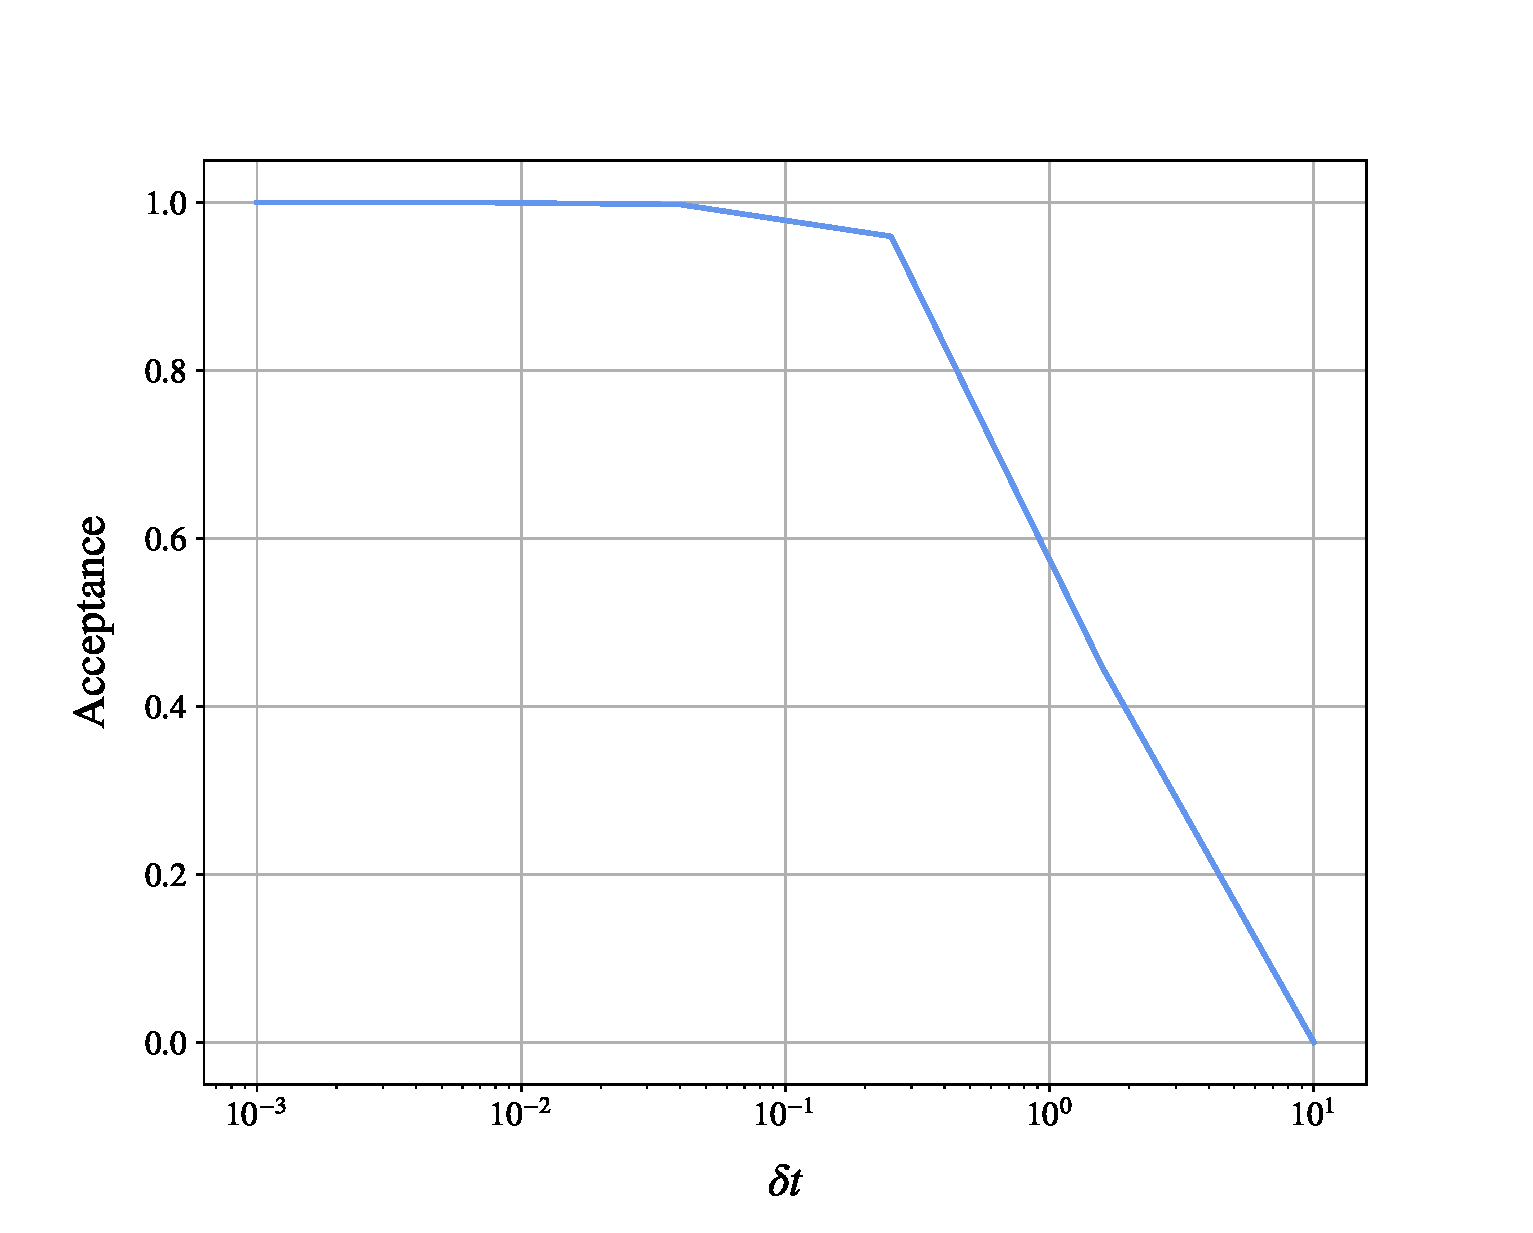
\includegraphics[scale=0.37]{images/varying_dt.eps}
    \caption{Acceptance ratio as a function of the time-step $\delta t$ in the context of VMC simulation performed with the importance sampling technique. Each run is conducted with $N_{therm}=10^5$, $N_{steps}=2^{21}$ and involves a system of $10$ non-interacting particles in 3-dimensions with $\alpha=0.5$.}
    \label{fig:dt_importance_sampling}
\end{figure}

\begin{figure}[H]
    \centering
    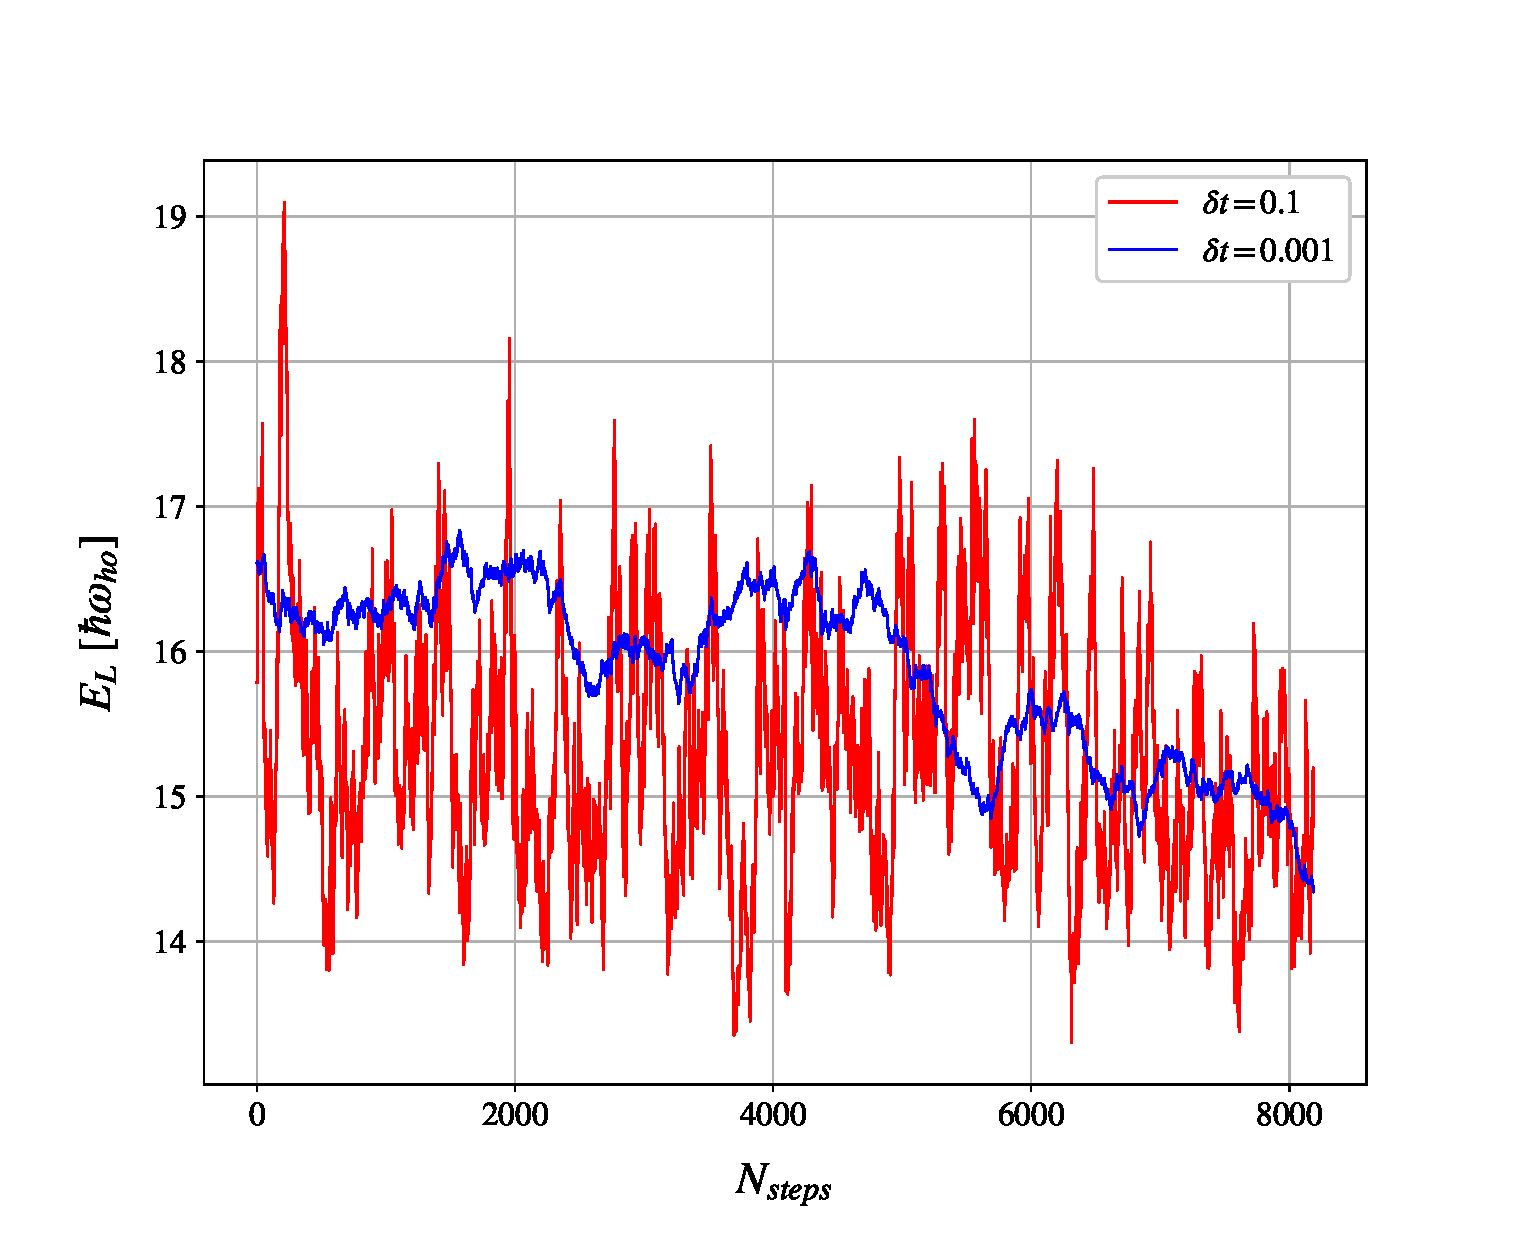
\includegraphics[scale=0.37]{images/correlation_different_deltat.eps}
    \caption{Local energy evaluated in each step of a VMC simulation after $N_{therm}=10^5$. A $3D$ system populated by 10 non-interacting particles inserted in a spherical potential is considered here. The image shows two curves for the chosen parameter $\delta t=0.001$ and $\delta t = 0.1$ used for the importance sampling method. The variational parameter $\alpha$ is set as constant to 0.4 to introduce some statistical fluctuations in the data, absent for $\alpha=0.5$. }
    \label{fig:correlation_varying_dt}
\end{figure}


\subsubsection{STATISTICAL ANALYSIS THROUGH BLOCKING METHOD}
As previously stated, Table \ref{tab:varying_alpha_noninteracting} contains estimations of the error affecting $\langle E_L(\alpha) \rangle$ obtained directly from the variance provided by the VMC simulations and the one obtained with the blocking technique. The python script that provided us with these latter results is based on the theoretical background described in Section \ref{sec:blocking_method}. The consistency of the mentioned script was also tested, in particular for what concerns the convergence of the estimate for  $\sigma_\mu^2$ (see Eq.\,\ref{eq:blocking_method}) to a finite value after a sufficiently high number of blocking iterations. In Figure \ref{fig:blocking_analysis} we present the values of $\sigma_k$ after each iteration of the mentioned method: the results are derived from a simulation performed with $2^{23}$ steps on a $3D$ system containing $N=10$ non-interacting particles inserted in a spherical potential. The sampling was performed through the Metropolis-Hastings algorithm using $\delta t=0.1$ and the variational parameter was again set to $\alpha=0.4$. As expected, we can observe that $\sigma_k$ reaches a plateau for sufficiently high values of $k$, and then an erratic behaviour enters into play, this due to the progressive reduction of the amount of points on which the variance is estimated. 

\begin{figure}[H]
    \centering
    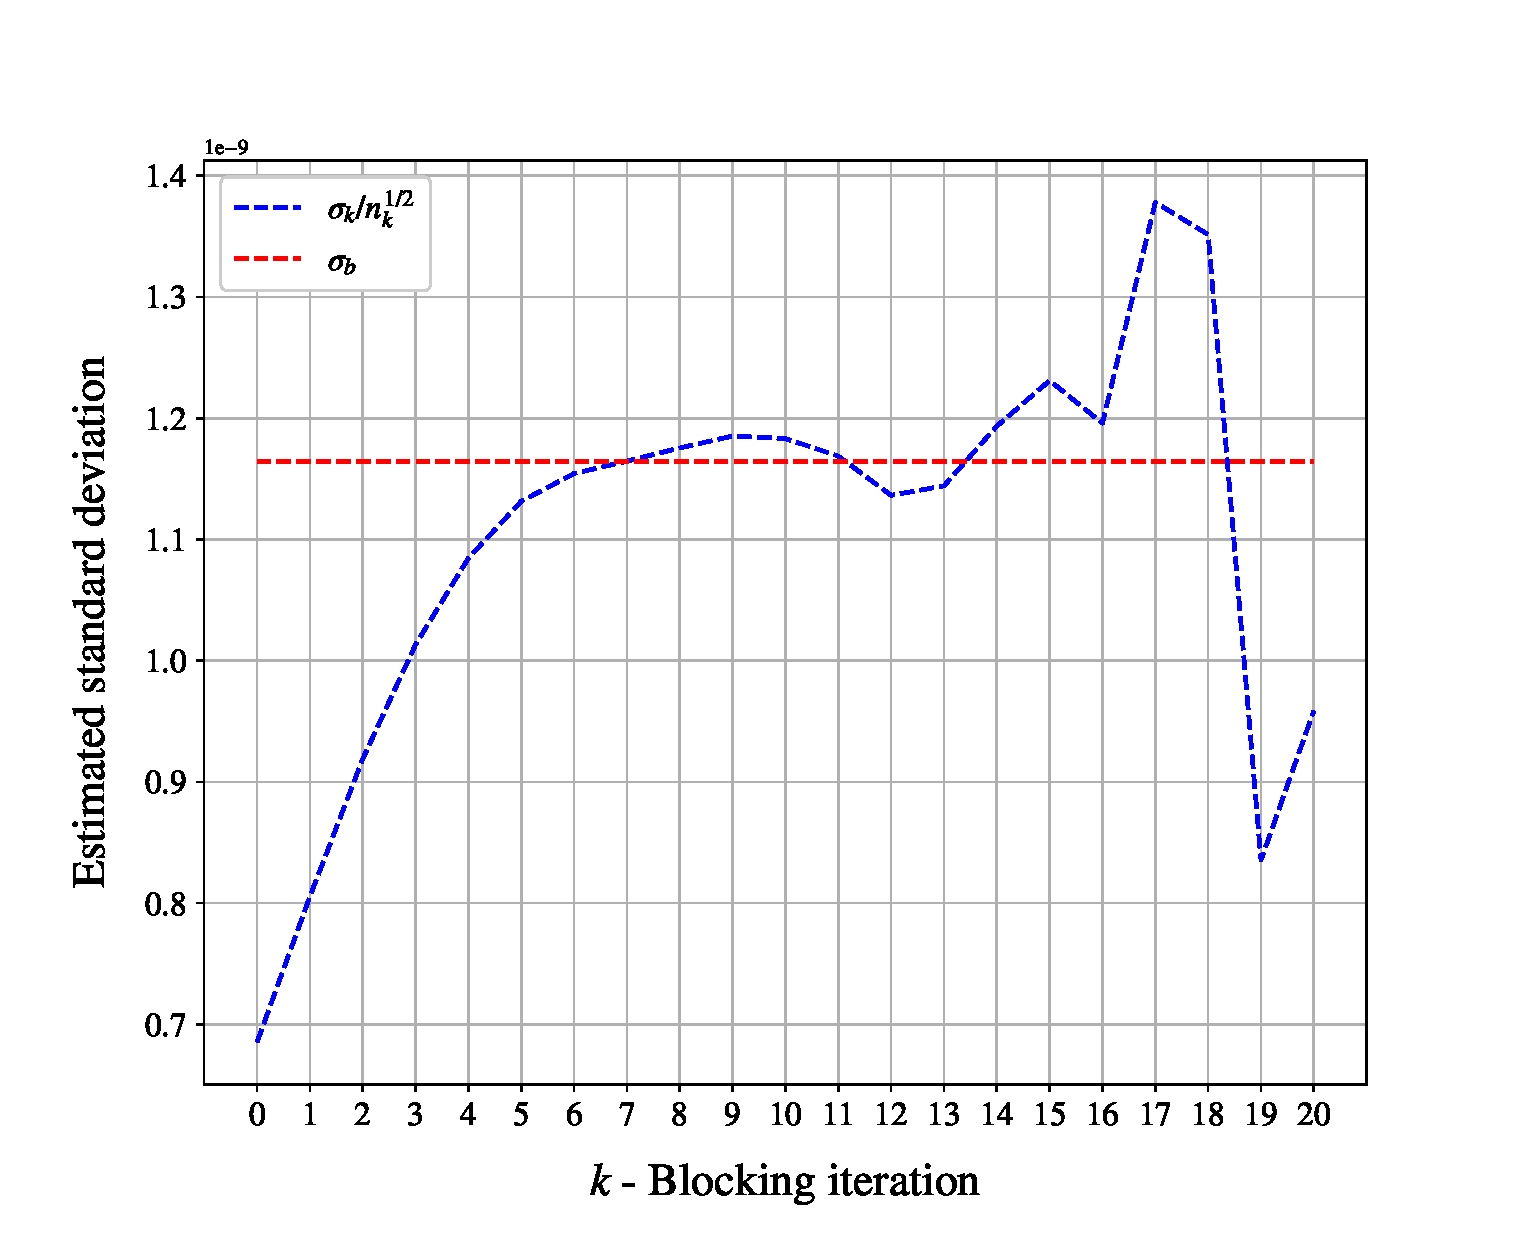
\includegraphics[scale=0.37]{images/sigma_blocking_behaviour.eps}
    \caption{The figure shows the behaviour of the variance estimate provided by the blocking technique implemented in a python script. The simulation was performed with $N_{therm}=10^5$ and $N_{steps}=2^{23}$ on a non-interacting $3D$ system characterized by $\alpha=0.4$ and populated by 10 particles. The Metropolis-Hastings algorithm with $\delta t =0.1$ was adopted for the sampling. }
    \label{fig:blocking_analysis}
\end{figure}


\subsection{INTERACTING CASE}
Subsequently we moved on to the interacting and asymmetrical case with trial wavefunction given by Eq.\,\ref{wavefunctions} and Hamiltonian described in Eq.\,\ref{hamiltonian} and Eq.\,\ref{elliptical_pot}. At first we compared results with those obtained from the symmetrical case, again to test the solidity of our code: this could be done by setting $\beta=1$, $w_z = w_{ho} = 1$ and the s-wave scattering length $a$ to 0. We verified that the results were coincident with those obtained in the non-interacting case, using both the Brute-force Metropolis algorithm and the importance sampling (see Appendix \ref{appendix:interacting_reduced_as_non_interacting}). From now on we will omit to specify the sampling algorithm used for each simulation, since all the next results were derived exploiting the Metripolis-Hastings one: this choice was driven by the fact that the this technique provides the combination of a higher acceptance ratio and better statistical sampling of the data. Furthermore, the variance on the energy value provided by each VMC was estimated through the blocking analysis. From now on, this information will be omitted too. \\

After the aforementioned consistency check we set the parameters' values $\omega_z = \beta = 2.82843$ and $a = 0.0043$ and ran the simulations for $N=10,50,100$ particles while varying $\alpha$. The simulations for 10 and 50 particles were carried out using $2^{21}$ steps, while in the case of 100 particles the high computational time imposed us a reduction of the number of steps to $2^{19}$. The parameter $\delta t = 0.1$ was the same for every run and the corresponding results are reported in Table \ref{tab:varying_alpha_noninteracting}. Furthermore, as an example the results obtained for 10 particles are reported in Figure \ref{fig:asymm_symm_comparison}, compared with their homologous obtained in the non-interacting symmetrical case. Figure \ref{fig:E_over_N} reports a comparison between the energy per particle as a function of the variational parameter $\alpha$ obtained for the three different values of $N$. \\



\begin{table}[H]
    \centering
    \begin{tabular}{cccc}
    \toprule
        \multicolumn{4}{c}{$N=10$} \\
        \midrule
        $\alpha$ & $\langle E_L \rangle$ & $\sigma_B$ & acc.ratio \\
        \midrule
        $0.3$ & 27.59 & 0.02 & 0.98185 \\
        $0.4$ & 24.969 & 0.008 & 0.97230 \\
        $0.5$ & 24.3991 & 0.0003 & 0.96178  \\
        $0.6$ & 24.822 & 0.006 & 0.94964 \\
        $0.7$ & 25.83 & 0.01 & 0.93758 \\
        \midrule
        \midrule
        \multicolumn{4}{c}{$N=50$} \\
        \midrule
        $\alpha$ & $\langle E_L \rangle$ & $\sigma_B$ & acc. ratio \\
        \midrule
        $0.3$ & 142.8 & 0.1 & 0.97840 \\
        $0.4$ & 129.81 & 0.04 & 0.96866 \\
        $0.5$ & 127.287 & 0.006 & 0.95759 \\
        $0.6$ & 129.90 & 0.03 & 0.94583 \\
        $0.7$ & 135.54 & 0.06 & 0.93361 \\
        \midrule
        \midrule
        \multicolumn{4}{c}{$N=100$} \\
        \midrule
        $\alpha$ & $\langle E_L \rangle$ & $\sigma_B$ & acc. ratio \\
        \midrule
        $0.3$ & 296.8 & 0.4 & 0.97610 \\
        $0.4$ & 271.2 & 0.1 & 0.96336 \\
        $0.5$ & 266.51 & 0.07 &  0.93323\\
        $0.6$ & 272.8 & 0.2 &   0.94392\\
        $0.7$ & 285.1 & 0.2 &  0.92906\\
        \bottomrule
    \end{tabular}
    \caption{The table reports the results of the simulations for different values of the variational parameter $\alpha$ for a $3D$ system constituted by $N=10,\;50,\;100$ particles. The simulations were performed exploiting the Metropolis-Hastings algorithm with $\delta t=0.1$, $N_{therm}=10^5$ and $N_{steps}=2^{21}$ for $N=10,\;50$, while and $N_{steps}=2^{19}$ for $N=100$. }
    \label{tab:varying_alpha_interacting}
\end{table}


\begin{figure}[H]
    \includegraphics[scale=0.37]{images/varying_alpha_comparison_interacting_and_not.eps}
    \caption{The figure reports the energy estimates as a function of $\alpha$ generated by various VMC simulations exploiting the importance sampling algorithm with $N_{therm}=10^5$, $N_{steps}=2^{21}$, $\delta t = 0.1$. The curves are referred to a $3D$ system populated respectively by 10 non-interacting particles in a spherical potential and 10 interacting particles in an elliptical potential. The errorbars are too small to be seen. }
    \label{fig:asymm_symm_comparison}
\end{figure}


\begin{figure}[H]
    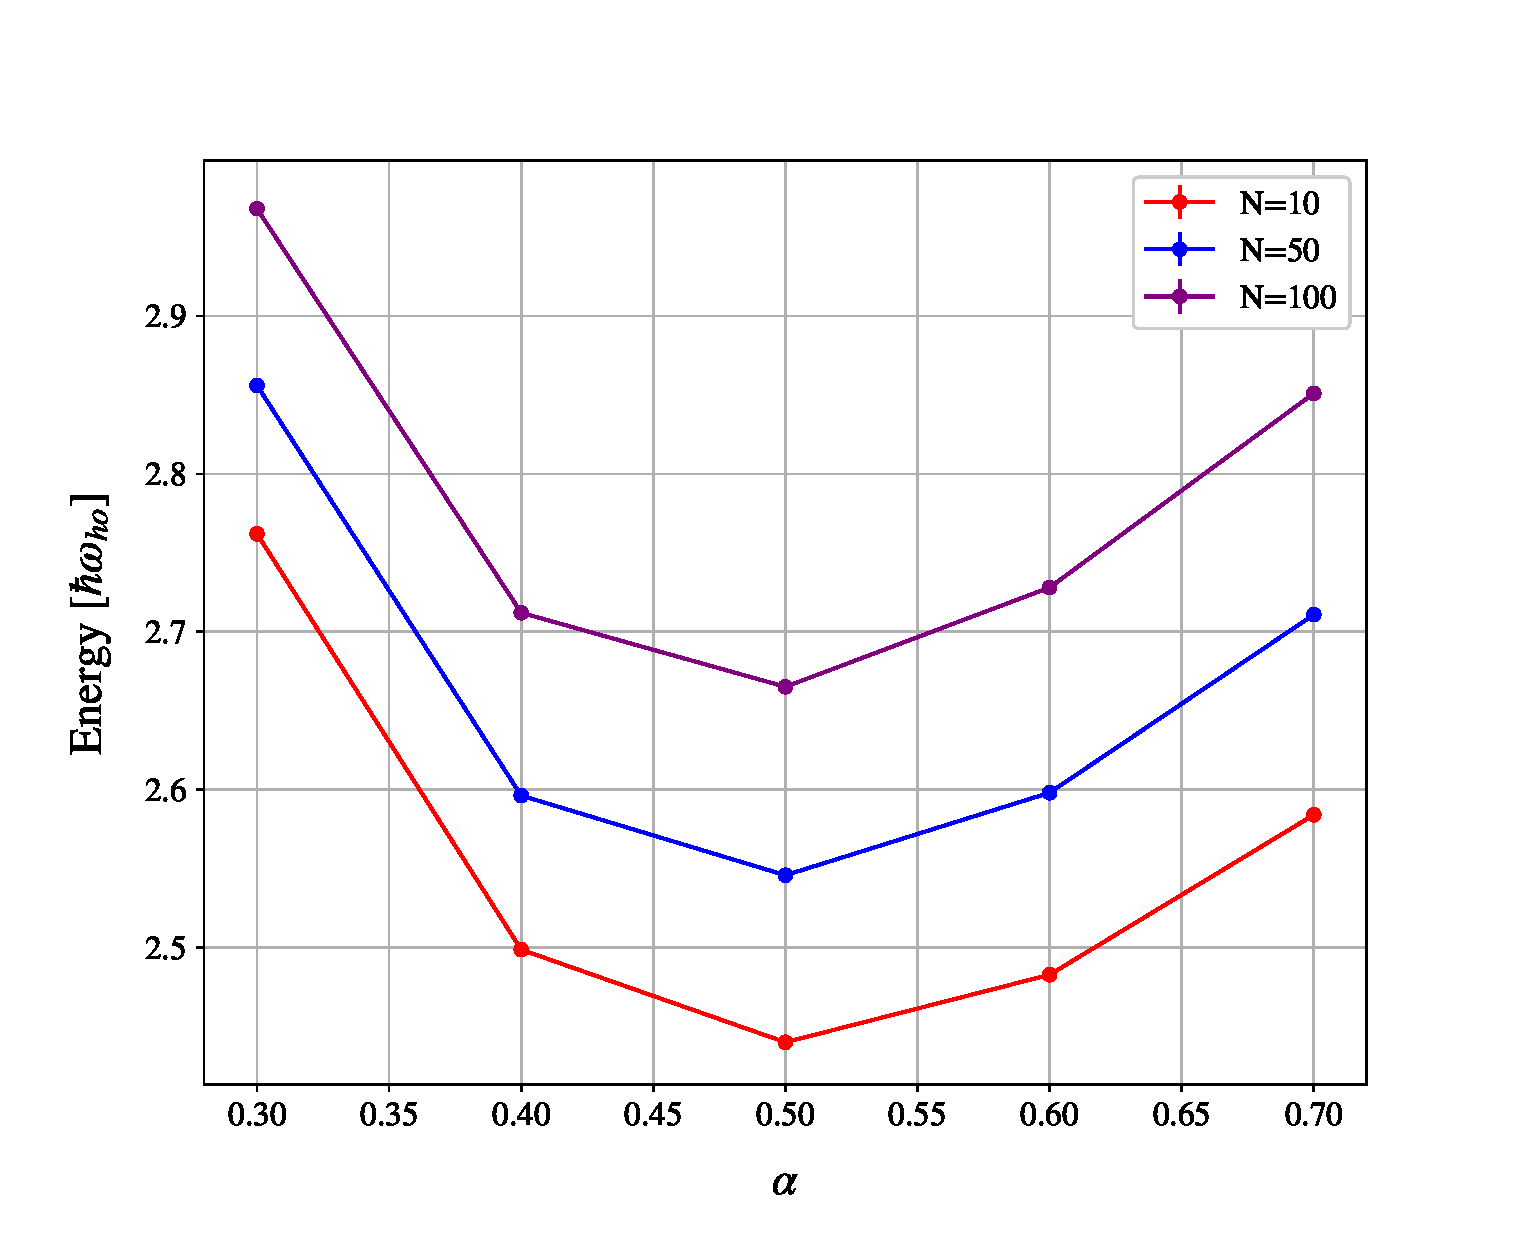
\includegraphics[scale=0.37]{images/energy_over_N.eps}
    \caption{The figure reports the average energy per particle as a function of $\alpha$ generated by various VMC simulations exploiting the importance sampling algorithm with $N_{therm}=10^5$ and $\delta t = 0.1$. The curves are referred to a $3D$ system populated respectively by 10, 50 and 100 interacting particles in an elliptical potential. The number of employed steps was $2^{21}$ for $N=10$ and $N=50$, while $2^{19}$ for $N=100$. }
    \label{fig:E_over_N}
\end{figure}


\subsection{GRADIENT DESCENT}
\label{sec:gradient_descent_results}
When considering the interaction between particles, the proof of the convexity of the function describing $\langle E_L \rangle$ as a function of $\alpha$ is non-trivial, thus in principle we can not state with absolute confidence that the curve is convex. However, as we can see from the latest figures, the behaviour of $\langle E_L \rangle$ as a function of $\alpha$ still encourages us to exploit the gradient descent method to research for  $\alpha_{GS}$ which minimizes the energy of the system. Before proceeding with the actual investigation in the interacting case, we tested the correct functioning of our code by applying it to a non-interacting system. In this simple case, it is well known that the optimal value of the variational parameter is $\alpha_{GS}=0.5$ and this result is independent of the number of particles and dimensionality. Therefore we expect to reach a convergence to this value whatever the adopted configuration. In particular, when considering particles without interaction we have at our disposal the analytical expression for the total energy of the system (see Eq.\,\ref{energy_analitical}) and the convexity of it is easy to prove. This ensures us that, if the method is capable in reaching a convergence for a sufficiently small value of the so-called learning rate $\gamma$ appearing in Eq.\,\ref{alpha_k}, the gradient descent will lead to a proper estimation of $\alpha_{GS}$. Table \ref{tab:gradient_descent_noninteracting} reports the results obtained with the application of the gradient descent method to a 3-dimensional system of 1, 10 and 100 non-interacting particles. Each VMC run was performed with $\delta t=0.1$ and $10^5$ thermalization steps, followed by another $10^5$ for the actual evaluation of the quantities reported in Eq.\,\ref{dEnergy_dalpha}. The learning rate was properly chosen for each configuration and the tolerance on the derivative was fixed to $\varepsilon=10^{-8}$ with no limit on the maximum number of iterations. The stability of the algorithm was also tested by performing the descent starting from two different guesses for the variational parameter, namely $\alpha_0=0.4$ and $\alpha_0=0.6$.


\begin{table}[H]
    \centering
    \begin{tabular}{ccccc}
    \toprule
        $N$ & $\gamma$ & $\alpha_0$ & $\alpha_{best}$ & $N_{conv}$ \\
        \midrule
        1 & 1\e-2 & 0.4 & 0.500 & 285 \\
        1 & 1\e-2 & 0.6 & 0.500 & 295 \\
        10 & 1\e-2 & 0.4 & 0.500 & 21 \\
        10 & 1\e-2 & 0.6 & 0.500 & 23 \\
        100 & 1\e-3 & 0.4 & 0.500 & 24 \\
        100 & 1\e-3 & 0.6 & 0.500 & 26 \\
        \bottomrule
    \end{tabular}
    \caption{Convergence analysis for the energy minimization process performed on a $3D$ non-interacting system of 1, 10, 100 particles in a spherical potential. The simulations were performed with $10^5$ steps for both thermalization and actual run, adopting the importance sampling with $\delta t = 0.1$, adjustable $\gamma$ and tolerance $\varepsilon=10^{-8}$. $N_{conv}$ refers to the number of gradient descent steps to get to convergence and $\alpha_0$ is the initial guess selected for the variational parameter.}
    \label{tab:gradient_descent_noninteracting}
\end{table}


Switching now to consider the interaction between particles, in this case the problem was less trivial, since the optimal value of the variational parameter depends also on the chosen number of particles and on the starting value of $\alpha$. Moreover, contrarily to the previous case, the exact value of $\alpha_{GS}$ is unknown and thus our research must be even more rigorous. However, the major limitation to precision here is constituted by the evaluation of the derivative of $\langle E_L \rangle$ with respect to $\alpha$. In fact, running a simple gradient descent with 10 particles, $\alpha_0=0.4$ and $\gamma=10^{-3}$ we observed that after some steps the derivative started oscillating between positive and negative values, always similar in magnitude between each others. The stochastic evaluation of this derivative enters here: in fact, even increasing the number of steps for each simulation or reducing the learning rate, we did not observe a further reduction of the derivative. Its values were always oscillating around zero, without decreasing in magnitude. We therefore retained to implement the method as follows: in the parallelized version of the code, each tread hosted a full gradient descent and for each number of particles we performed a first descent by adopting $\gamma=10^{-3}$ for a rapid convergence to a proximity of the result we aim at. When the aforementioned derivative started showing its oscillatory behaviour, a smaller $\gamma$ was selected and combined with a higher number of steps for each VMC simulation, this with the aim of increasing the precision in the evaluation of the derivative. If with these two improvements the algorithm still provided us with the above described oscillatory behaviour, the descent was interrupted and the selected $\alpha_{GS}$ is the average between the last values provided by each of the cores. Again the single runs were performed for $N=10,\,50,\,100$ using $10^5$ VMC steps and $\delta t =0.1$. For each $N$ the research of the optimal variational parameter was performed starting from 2 initial guesses. Our analysis is resumed in Table \ref{tab:gradient_descent_interacting}.

Once that the values of $\alpha_{GS}$ has been achieved for any selected configuration, we proceeded with a final VMC run to estimate the ground state energy for each apparatus. The results reported in Table \ref{tab:final_GS_energy} are referred to simulations performed with $\delta t = 0.1$ and with a number Monte Carlo steps varying with the number of particles involved in the system (this choice was caused by the huge amount of time required for the simulations involving a highly populated system). We selected $2^{27}$ MC steps for $N=10$, $2^{25}$ MC steps for $N=50$ and $2^{23}$ MC steps for $N=100$. 


\begin{table}[H]
    \centering
    \begin{tabular}{cccccc}
        \toprule
        $N$ & $\alpha_{0}$ & $\alpha_{best}$ & $\gamma_{min}$ & $N_{steps-max}$ & $N_{conv}$ \\
        \midrule
        10 & 0.4 & 0.49751 & 1\e-3 & 1\e5 & 74 \\
        10 & 0.6 & 0.49751 & 1\e-3 & 1\e5 & 74 \\
        50 & 0.4 & 0.48881 & 1\e-5 & 2\e5 & 21 \\
        50 & 0.6 & 0.48939 & 1\e-5 & 2\e5 & 21 \\
        100 & 0.4 & 0.481 & 1\e-5 & 5\e5 & 16 \\
        100 & 0.6 & 0.483 & 1\e-5 & 5\e5 & 11 \\
        \bottomrule
    \end{tabular}
    \caption{Convergence analysis for the energy minimization process performed on a interacting system of 10, 50 and 100 particles in a elliptical potential. A detailed description of the algorithm implemented for reaching these results is described in Paragraph \ref{sec:gradient_descent_results}. Here $\gamma_{min}$ and $N_{steps-max}$ are the minimum learning rate and maximum number of VMC steps used to perform a single run, while $N_{conv}$ is the iteration number at which the algorithm was stopped. Each run was performed employing the importance sampling with $\delta t = 0.1$ and $N_{therm}=10^5$. }
    \label{tab:gradient_descent_interacting}
\end{table}


\begin{table}[H]
    \centering
    \begin{tabular}{ccccc}
    \toprule
            $N$ & $\alpha^{GS}$ & $E$ & $\sigma_B$ & acceptance \\
            \midrule
            10 & 0.49751 & 24.39843 & 0.00003 & 0.96234 \\
            50 & 0.4891 & 127.48 & 0.07 & 0.94926 \\
            100 & 0.482 & 266.38 & 0.04 & 0.95036 \\
            \midrule
        \end{tabular}
    \caption{Results obtained for the ground state energy of a system of interacting particles in an elliptical potential. The final estimates were derived through VMC runs using the importance sampling method with $\delta t = 0.1$ and $10^{5}$ thermalization steps. We selected $N_{steps}=2^{27}$, $N_{steps}=2^{25}$ and $N_{steps}=2^{23}$ respectively for the systems in each of the 3 configurations with 10, 50 and 100 particles. The simulations were carried out exploiting the optimal variational parameter found after the gradient descent minimization and reported in Table \ref{tab:gradient_descent_interacting}. }
    \label{tab:final_GS_energy}
\end{table}




\subsection{ONE-BODY DENSITY}
With the energy-minimizing variational parameter at our disposal, we proceeded with the last step of our analysis, that is the previously introduced evaluation of the one-body density. Figure \ref{fig:one_body_density_histogram} shows the results obtained with the procedure described in section \ref{sec:one_body_density} applied to a system populated by 10 particles. For the construction of the curves reported below, the trial wavefunction of Eq.\,\ref{wavefunctions} was considered both with and without the Jastrow factor, varying the value of the parameter $a$ to amplify the effects introduced by the interaction term. In Figure \ref{fig:spatial_distribution_x_z} we represent also the spatial distribution of the particles along the $x$ and $z$ directions, in order to show the effects introduced by the modifications of the trap shape. The curves are referred to a system populated respectively by 10, 50 and 100 particles. Each of the simulations performed for this section were carried out with $\delta t = 0.1$ and $2^{23}$ steps, setting the $\alpha$ value to those reported in Table \ref{tab:final_GS_energy}.


\begin{figure}[H]
    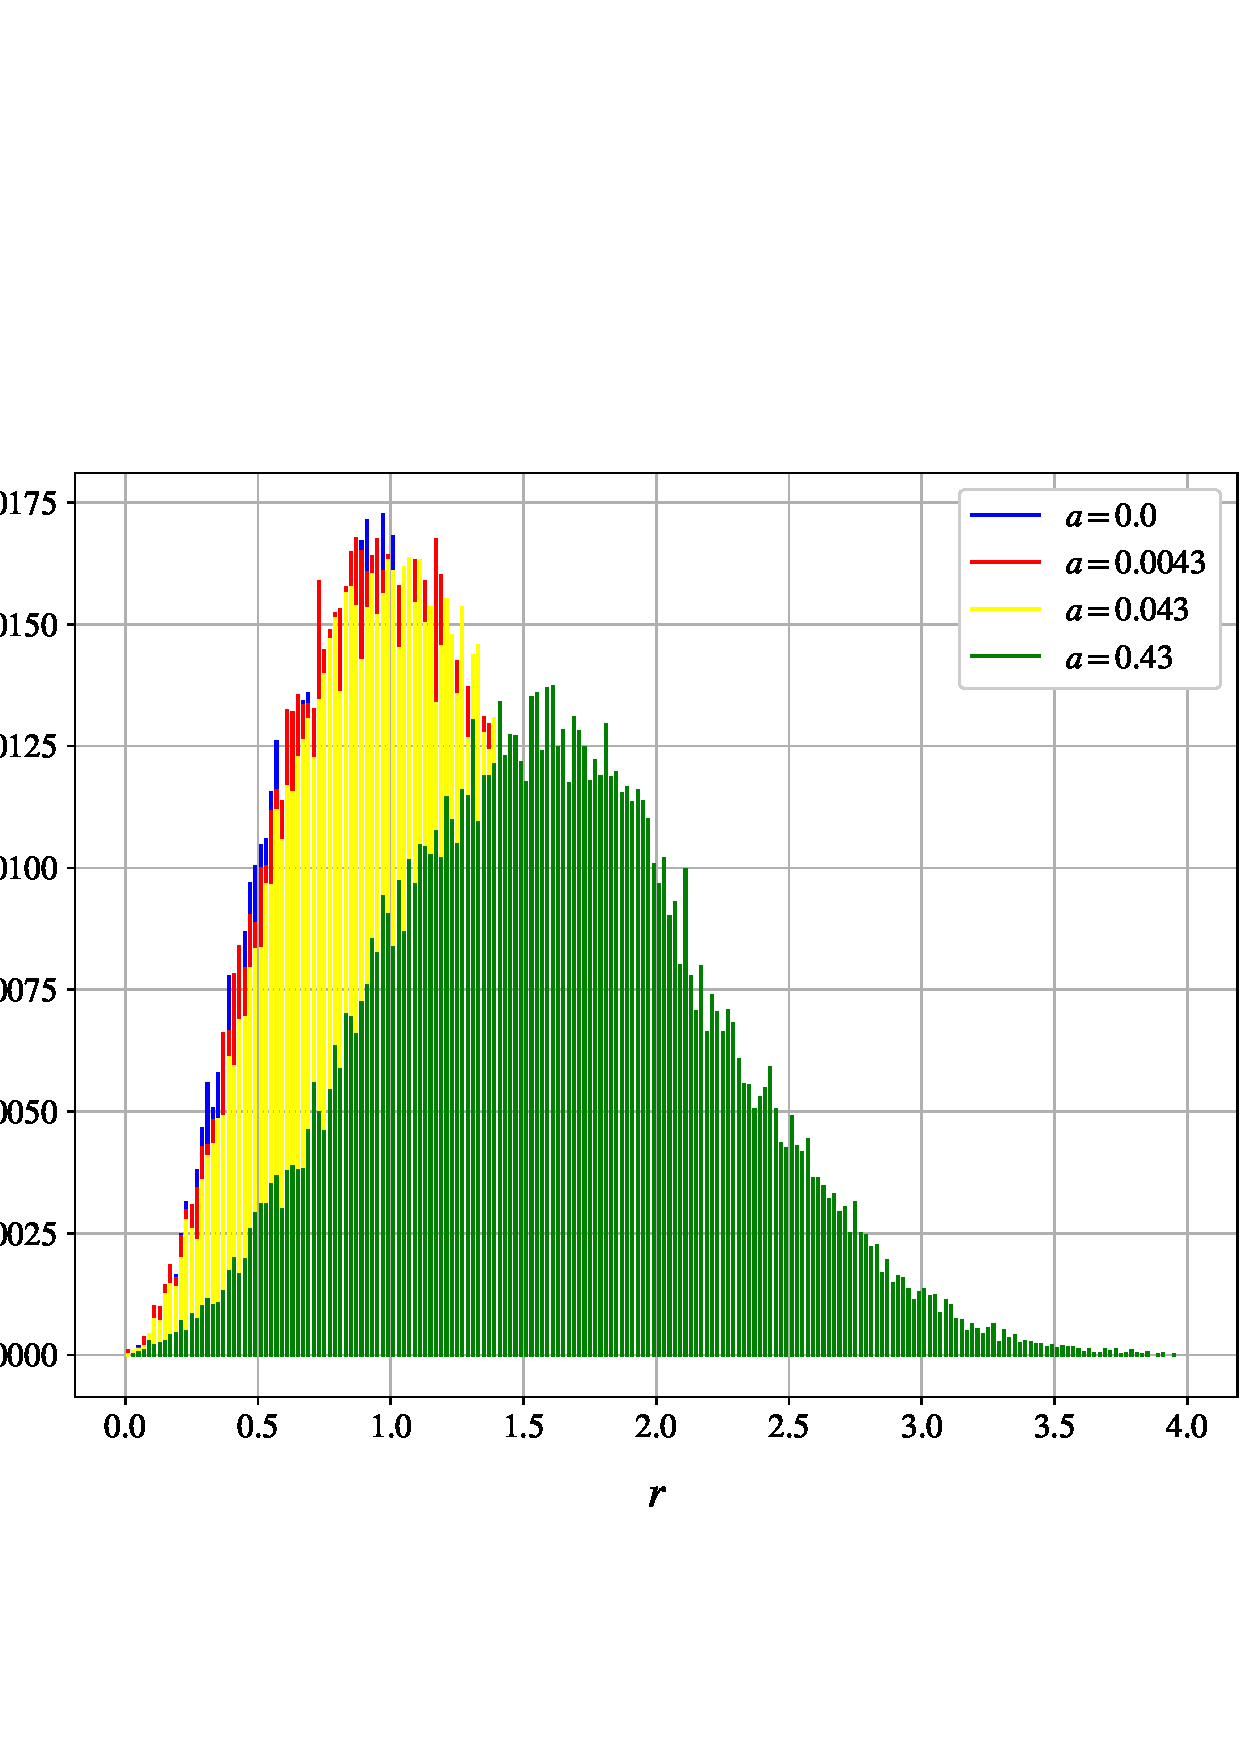
\includegraphics[scale=0.37]{images/onebody_density.jpg}
    \caption{One-body density as a function of the radial distance from the center of the chosen reference frame for a $3D$ system with $N=10$ particles described by an asymmetric gaussian wavefunction and inserted in a elliptical potential. The histograms are built for different values of $a$ in order to increase the effects introduced by the Jastrow factor in the wavefunction. The simulations were carried our exploiting the importance sampling with $N_{therm}=10^5$, $N_{steps}=2^{23}$, $\delta t =0.1$ and the $\alpha$ value deriving from the minimization of the energy (reported in Table \ref{tab:gradient_descent_interacting}). Notice that the curves for $a=0$ and $a=0.0043$ are almost perfectly overlapped. }
    \label{fig:one_body_density_histogram}
\end{figure}

\begin{figure}[H]
    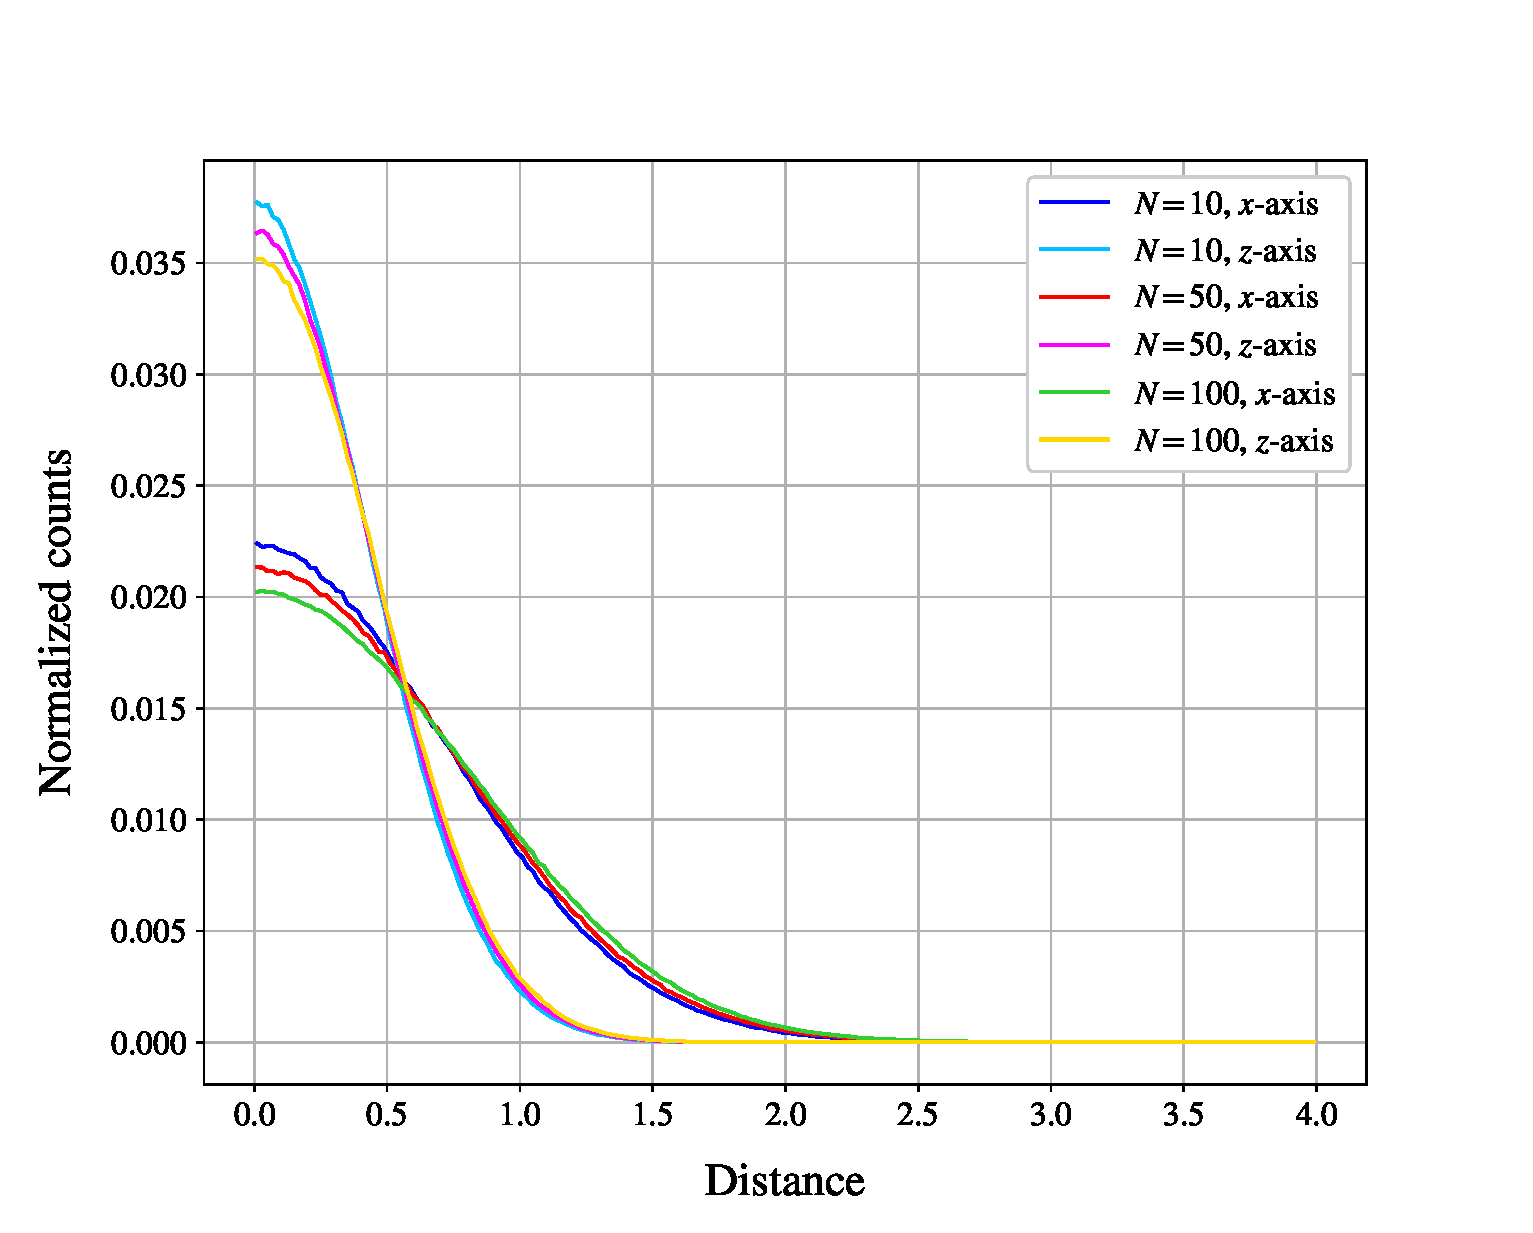
\includegraphics[scale=0.37]{images/spatial_distribution_x_z.eps}
    \caption{Particles' spatial distribution along the coordinates $x$ and $z$ for a system populated respectively by 10, 50 and 100 particles described by an asymmetric gaussian wavefunction and inserted in a elliptical potential. The simulations were carried our exploiting the importance sampling with $N{therm}=10^5$, $N_{steps}=2^{23}$ steps and $\delta t =0.1$, setting $\alpha$ to the values reported in Table \ref{tab:gradient_descent_interacting}. }
    \label{fig:spatial_distribution_x_z}
\end{figure}

\section{DISCUSSION ABOUT THE RESULTS}
\label{sec:discussion}
We start now the discussion about the results starting from those obtained for systems of non-interacting particles in a spherical potential. This simple case is analytically solvable, in the sense that the analytical expressions for all the quantities involved in this project can be found. Thus in principle a VMC approach could be avoided, but we still adopted this system for the sake of testing the implemented algorithms that would have been applied in a second moment to the interacting case. 

It is well known that the value of the variational parameter minimizing the energy of a non-interacting system considered in this project is $\alpha_{GS}=0.5$, independently on the degrees of freedom involved in the system. This is furthermore validated by Table \ref{tab:tab_x_metropolis_analytical} and Table \ref{tab:tab_x_metropolis_numerical}, reporting data produced with the brute-force Metropolis algorithm. As previously stated, the simulations exploiting the numerical approach were performed just for a comparison in precision and CPU time with the same simulations performed using analytical formulas, but they were of any practical use for this project. However, one can notice that the adoption of the numerical approach for the evaluation of the second derivative appearing in Eq.\,\ref{local_energy} produces less precise results, namely $\sigma_E$ is non-null, on the contrary of what happens when the local energy is evaluated analytically. Moreover, the CPU time is also drastically increased when the numerical approach is adopted. A more interesting aspect to notice is the behaviour of the acceptance ratio as a function of the dimensionality of the system. While using the brute-force Metropolis algorithm, the step size for generating the new proposal for each coordinate of the particles' position vector was always kept constant for all the possible tested configurations. This reflects on the acceptance ratio, which diminishes when the dimension $D$ of the apparatus grows. In fact, with the just mentioned choice for $r_{step}$ we are implicitly allowing a particle to move at each step up to a distance $r_{step} \ast \sqrt{D}$ apart from its previous position. As $D$ increases, particles can undergo larger movements and thus they are also more likely to end more distant from the origin, with a higher rejection probability for that move. \\

The considerations about precision and CPU time apply also to the simulations for $\alpha=0.5$ performed using the importance sampling algorithm, whose results are reported in Table \ref{tab:tab_x_importance_analytical} and Table \ref{tab:tab_x_importance_numerical}. The computational time spent on the single VMC runs performed here is slightly higher than the corresponding one needed for the analogous simulations employing the brute-force approach. This was expected too, since the importance sampling requires also the Greens' functions to be evaluated apart from the wavefunctions in order to discriminate between acceptance and rejection of a single move. Despite this little the inconvenient, the advantages brought by this second algorithm legitimate its implementation. The bias introduced by the drift force term in the proposal for a new move drives the system to high-probability states, leading thus to a higher acceptance ratio and to a better sampling in the high-probability regions of the space of configurations, which are those that more matter for statistics. \\


Once that the most basic features of our code were tested, we switched to a more information-providing case, that is $\alpha\neq 0.5$. Plots appearing respectively in Figure \ref{fig:varying_alpha_noninteract_metropolis} and Figure \ref{fig:varying_alpha_noninteract_importance} show the almost perfect overlap between the experimental points and the theoretical curve, remarking again the efficacy of VMC simulations in reproducing the expected behaviour. Furthermore, adopting $\alpha\neq0.5$ brought us away from the trivial case of null error on the estimated energy of the system. In fact, substituting $\alpha=0.5$ into Eq.\,\ref{local_energy_analytic_noninteracting}, one completely eliminates the dependence from the position of the particles, thus $E_L$ sampled along a VMC simulation assumes always the same value. On the contrary, with $\alpha\neq0.5$ the dependence of the local energy from $\bm{R}$ is reintroduced, bringing up some more meaningful statistics in the acquired data. This was also the occasion for a first encounter with the error estimation through the blocking method, which allowed us also to access the impact of correlation in the acquired measurements. Table \ref{tab:varying_alpha_noninteracting} reports some evaluated quantities in this sense: combining data from Figure \ref{fig:dt_importance_sampling} with the column referred to $\sigma_B$ helped us in tuning the parameter $\delta t$ for the successive VMC runs. We noticed that choosing a too small $\delta t$ introduced more correlation in the generated data, since the particles are less likely to be moved far away from their current position and thus more VMC cycles are needed to reach a sufficient degree of uncorrelation. For these reasons, $\delta t=0.1$ was chosen for the successive simulations, making large steps more suitable for the particles, still keeping a high acceptance ratio as typical for the importance sampling. The content of Figure \ref{fig:blocking_analysis} is reported to testify the correct behaviour of the python script used for the blocking analysis and is also a good instrument for a better comprehension of its functioning. As expected, the provided error estimate increases at each blocking iteration since always a larger fraction of the correlation term in Eq.\,\ref{err_covariance} is taken into account. After a certain number of iterations, a plateau is reached and then an erratic behaviour comes into play, due to the lack of data on which the variance is being evaluated. \\

The analysis of the non-interacting case acted as a springboard for the introduction of the interaction term between the particles. This new framework involved a system of 1, 50, 100 particles inserted in a elliptical potential and described by an asymmetric gaussian wavefunction multiplied by a Jastrow factor, as illustrated Eq.\,\ref{wavefunctions}. The investigations in this case became much less trivial, since an analytic solution for the energy of the system as a function of $\alpha$ is not available for any comparison. Moreover, the simulations became also much more time demanding due both to the complexity of the analytical formulas included in the code (e.g. Eq.\,\ref{local_energy_analitic_interacting}) and to the introduction of new computational elements which played a fundamental role in the evaluation of the needed quantities (i.e. the matrices containing information for the relative positions and distances described in Section \ref{sec:matrix_relative_dist}). These factors imposed a much more careful costs/benefits analysis before launching each simulations, especially a compromise had to be found between computational time and precision achieved for the results. 

A first example of this kind of decision was found with the evaluation of the energy of the system for a bunch of $\alpha$ values, as shown in Table \ref{tab:varying_alpha_interacting}. The simulations involving a group of 100 particles were clearly the most demanding: despite ideally a VMC simulation performed on this system would require a higher amount of steps than a simulation performed on a less populated environment, looking at the problem from a time-saving perspective we choose to employ less steps for this kind of run. Though, the selected number of steps allowed allowed us to keep a sufficiently low relative error on the energy estimation as a function of $\alpha$. In any case, data contained in the mentioned table provide a lot of pieces of information for what concerns the features of the new systems. In particular, one can see that the modifications added to both the hamiltonian and the wavefunction obviously changed the $\alpha$-dependence for the expected energy value, but the new $\alpha_{GS}$ which minimizes the energy of the system is still included in the interval $(0.4, 0.6)$ for every analyzed $N$. This fact is proved for the case of $N=10$ by the graph of Figure \ref{fig:asymm_symm_comparison}: here we can see the great impact introduced by the modifications applied to the system with respect to the non-interacting case. The two curves show a similar shape, with the clear presence of a minimum around $\alpha=0.5$, but the energy values related to our new configurations are always higher than those corresponding to a bunch of independent particles. This behaviour is completely reasonable, since now the trap is steeper in the $z$ direction and simultaneously the inter-particles distance must be higher than the typical s-wave scattering length $a$. 

A graphical representation of the content of Table \ref{tab:varying_alpha_interacting} is presented in Figure \ref{fig:E_over_N}. Another interesting fact is highlighted here: in the case of non-interacting particles, we experienced that the energy of the system resulted to be simply proportional to the number of particles and the dimensionality of the system, as suggested also in Eq.\,\ref{energy_analitical}. Here instead the aforementioned plot suggests that the interaction term appeared in the Hamiltonian has introduced a stronger dependence in the energy on the number of particles populating the system. This tendency is also shown in \cite{duBois}. Unfortunately the article focuses on systems populated by higher number of particles than those that we employed, thus a more precise comparison was not affordable. Back to our case, if the interaction between the particles is switched off (i.e. one sets $a=0$) the three curves of the mentioned figure would be almost perfectly overlapping (modulo stochastic fluctuations deriving from the VMC run), while when the interaction is considered they appear as clearly distinguished. This fact is again extremely reasonable, since, considered the repulsive interaction between the particles, increasing the population of the system will lead to a larger average distance from the origin and thus to a larger average energy per particle. \\

After all these preliminary considerations on the interacting system, we passed to the research of the $\alpha$ value which minimizes the energy. Results shown in Table \ref{tab:gradient_descent_noninteracting} come from the application of the gradient descent method to a non-interacting system with different number of particles: this kind of experiment was used to test the correctness of the code implementation, exploiting again the knowledge of the true value of $\alpha_{GS}$. For every case presented in the table, the descent proceeded without any issue or strange behaviour up to convergence. Once that the program was launched, the values of $\langle E_L \rangle$ described a monotonic decreasing function towards the minimum, with the corresponding derivatives with respect to $\alpha$ always decreasing in modulus down to the fixed tolerance. A much more interesting and also more demanding task is the research of this parameter in the interacting case, for which the only preliminary knowledge regards the range in which to search for it, namely $\alpha\in(0.4, 0.6)$, as suggested by Figure \ref{fig:E_over_N}. Contrarily to what happens for the non-interacting case, here we do not have at disposal a straightforward way to possibly demonstrate the convexity of $\langle E_L \rangle$ as a function of $\alpha$. However, again the shape of the curves reported in Figure \ref{fig:E_over_N} encourages us to apply the gradient descent method. 

In this much more complicated case, we had to face with a problem arising from the stochastic evaluation of the energy derivative with respect to $\alpha$. Our initial intent was to make a first descent to reach the proximity of the ground state energy and then proceed by choosing a smaller value of the parameter $\gamma$ appearing in Eq.\,\ref{alpha_k} in order to perform a finer search. However, the reduction of the learning rate revealed to be insufficient to guarantee the correct continuation of the descent, since the fluctuations in the derivative values were too large. Two different single VMC runs performed in the same conditions and with the same value for $\alpha$ could produce two estimates for $d\langle E_L \rangle / d\alpha$ close to zero, but maybe differing also in the sign. A possible solution to get rid of this inconvenient could consist in increasing the number of steps employed for each simulation along the descent, hoping that this could lead to a better estimation of the derivative, but again we had to find a compromise between computational time and precision in the results. So we decided to proceed by implementing the gradient descent as already described in Section \ref{sec:gradient_descent_results}. The results derived from these procedures appear in Table \ref{tab:gradient_descent_interacting}: one can notice that the number of gradient descent iterations that were necessary to reach the reported results decreases as the number of particles in the system grows. This is due to the fact that for larger $N$ the magnitude of the fluctuations in the derivative increased, thus limiting the descent to a few steps. 

For all the simulations performed in the context of gradient descent, we observed the extreme sensitivity of the method to the initial guess for $\alpha$, the value of the learning rate and the number of steps performed in each MC simulation. \\

Table \ref{tab:final_GS_energy} shows that the estimated values of $\alpha_{GS}$ decrease as N increases, confirming again that adding particles to the configuration contributes to move away the system from the non-interacting approximation treated before. The simulations with the final estimates of $\alpha_{GS}$ for 10, 50 and 100 particles populating the systems were finally performed and the corresponding results are still in Table \ref{tab:final_GS_energy}. For this kind of simulations the number of steps was higher than the average amount used for the other runs treated in the project, since we aimed to reach an accurate estimation of the ground state energy of the system.

Using a even higher number of particles would have lead to a non-affordable computational time for our devices, but a result for $N=500$ was found in \cite{Nilsen2005}. In this case the value found was $\alpha_{GS}=0.475$, confirming the tendency just described for $\alpha_{GS}$.  \\

As a final remark, the one-body density plotted in Figure \ref{fig:one_body_density_histogram} for a bunch of $a$ values tells us about the role played by the repulsive interactions in determining their radial distribution in the system. As the minimum allowed distance between the particles increases, we can see a clear tendency to occupy positions further from the origin of the system. Here we find another evidence of what discussed above about the role played by the repulsive interaction: in principle the particles tend to occupy positions close to the origin of the system, in order to minimize its energy, but here they are forced to have reciprocal distance larger than $a$. Two of them are thus forbidden to be simultaneously close to the origin. The figure shows that an increase in the value of $a$ leads to an increase in the average distance from the origin, despite the particles have to face with a steeper potential.

The introduction of the elliptical trap caused the particles to be more confined along that direction, as shown in Figure \ref{fig:spatial_distribution_x_z}. In addition, this graph constitutes a further confirmation of the fact that adding more and more particles to the system brings it always less comparable to a non-interacting one. As a matter of fact, in this simpler case the average dispersion of the particles along a specific direction wouldn't be influenced by the number of elements appearing in the system, contrarily on what happens when the interaction in taken into account. Here we see again that a larger population leads to a greater dispersion of the particles with respect to the origin of the system. The same statements are reported also in \cite{duBois}, but here the observations are again focused on systems with thousands of particles in them. 








\section{POSSIBLE FURTHER IMPROVEMENTS}
\label{sec:improvements}
The code has been built since the beginning as a fully object-oriented program, defining thus a clear and well organized structure suitable also for further applications to other systems. New sub-classes can in principle be added to the primary ones, allowing the user to approach other problems in the context of Quantum Mechanics. \textcolor{red}{The speed of the code can also be enhanced by the adoption of libraries pointed towards scientific computing (e.g. \texttt{<armadillo>}), but this would probably require heavy modifications to the already implemented structure.} 

A finer research of the $\alpha$ value which minimizes the energy of the system could be achieved substituting the very rough standard gradient descent with an improved version of it (e.g. stochastic gradient or conjugate gradient), maybe also exploiting some built-in python functions to approximate the Hessian matrix needed for the implementation. 


\section{CONCLUSIONS}
\label{sec:conclusions}
In the first part of the present project we tested the implementation of the code by applying it to describe a system of non-interacting bosons in a spherical trap. Both the VMC simulations based on the analytical and numerical evaluation of the local energy for $\alpha=0.5$ provided the expected results, the latter suffering a small lack of precision and requiring a much higher CPU time. Moreover, the algorithm exploiting the analytical formula for the local energy provided excellent results also for $\alpha\neq0.5$, following the expected behaviour described by the theoretical curve of $\langle E_L \rangle$ as a function of $\alpha$. The comparison of the results coming from the brute-force Metropolis algorithm and the Metropolis-Hastings one lead us to prefer the latter because of the higher acceptance ratio and the better sampling properties provided by it. The time-step was set to $\delta t = 0.1$, which allows for having a high acceptance ratio combined with a larger average step length for the particles. This leads also to a faster exploration of the possible configurations and in a reduction of the correlation between consecutive steps. 

Switching to the interacting case, we verified that by setting the parameters $\omega_z$, $\beta$ and $a$ in order to lead back to the non-interacting system, we achieved a last successful comparison with the known analytical results. The application of the gradient descent provided us with three values for the $\alpha$ minimizing the energy of the system, respectively $\alpha_{10}=0.49751$, $\alpha_{50}=0.4891$ and $\alpha_{100}=0.482$, showing a decrease as the number of particles $N$ increases (this tendency was also confirmed in \cite{Nilsen2005}). The fluctuations in the estimate for the $\alpha$-derivative of $\langle E_L \rangle$ came into play after a few iterations of the gradient descent, preventing us to reach a higher precision in the estimate of $\alpha_{GS}$. This precision actually decreases with increasing $N$, since the magnitude of the fluctuations increases too. The MC simulations performed with the estimated $\alpha_{GS}$ provided us with $\langle E_L \rangle_{10} = 24.39843 \pm 0.00003$, $\langle E_L \rangle_{50} = 127.48 \pm 0.07$ and $\langle E_L \rangle_{100} = 266.38 \pm 0.04$, with the uncertainties estimated through the blocking method. The error affecting the result for 100 particles is surely underestimated: this may be attributable to the smaller amount of steps employed for the final simulation, not allowing for a proper estimation of the error through the blocking method. The modifications to the Hamiltonian and the introduction of the Jastrow factor in the wavefunction influenced also the behaviour of the average energy per particle introducing a dependence on $N$, contrarily to what observed for independent particles in the non-interacting case. The hard-sphere potential lead also to an increase of the average distance between the particles and the origin, this fact appearing as a little modification in the shape of the one-body density. Also in this case, the modifications became more and more evident as the population of the apparatus increased. These evidences are confirmed by the results reported in \cite{duBois}, where larger populations are analyzed.

The combination of all these observations manifests the fact that when the interaction between particles is considered, a higher $N$ will make a possible approximation to the non-interacting case always less and less precise.
\end{multicols*}

\begin{multicols}{2}
\printbibliography
\end{multicols}

\newpage
\begin{multicols*}{2}
\section*{APPENDIX}
\appendix
\section{LOCAL ENERGY: ANALYTICAL FORM}
\label{appendix:local_energy}
This section is devoted to show the detailed analytical derivation of the local energy formula in the general case. All the specific cases can be gotten from the final result reported below by setting properly the parameters of the system. For the sake of notation, we remind that we set $m=\hbar=\omega_{ho}=1$ and we introduce the variable $\bm{r}$ as a cumulative variable for $\{\bm{R}, \alpha, \beta\}$. The trial wavefunction describing the most general configuration for the system is reported in Eq.\,\ref{wavefunctions}, however to better face the analytical derivation we rewrite it here as:
\begin{equation*}
    \Psi_T(\mathbf{r} )=\left[ \prod_i^N g(\alpha,\beta,\mathbf{r}_i) \right] \exp{\left(\sum_{j<m}u(r_{jm})\right)}
\end{equation*} 
with 
\begin{equation}
    u(r_{ik})=\ln (f_{ik}) = \ln \left( 1-\frac{a}{r_{ik}} \right)
    \label{app:u_interaction}
\end{equation}
and
\begin{equation}
    g(\alpha,\beta,\mathbf{r}_i) = \exp{\left[-\alpha(x_i^2+y_i^2+\beta
    z_i^2)\right]}= \phi(\mathbf{r}_i)
    \label{app:gaussian}
\end{equation} 
The Hamiltonian of the system acquires the following form: 
\begin{equation*}
    \hat{H} = \frac{1}{2} \sum_i^N \left( - \nabla_{i}^2 + x_i^2 + y_i^2 +  \omega_{z}^2 z_i^2 \right) 
    +\sum_{i<j}^{N} V_{int}({\mathbf{r}}_i,{\mathbf{r}}_j)
\end{equation*}
We consider the %non trivial 
case of $r_{ij}>a,\, \forall i,j$, then  $V_{int}(\mathbf{r}_i,\mathbf{r}_j) = 0$. According to the definition of the local energy, we get
\begin{align}
    E_L(\mathbf{r}) &= \frac{1}{\Psi_T(\mathbf{r})} \hat{H} \Psi_T(\mathbf{r}) \nonumber\\
    &= -\frac{1}{2} \sum_k^N  \frac{\nabla_{k}^2\Psi_T(\mathbf{r})}{{\Psi_T(\mathbf{r})}} +\sum_k^N \frac{1}{2} \left(x_k^2 + y_k^2 + \omega_{z}^2 z_k^2 \right) 
    \label{app:localenergy_appendix}
\end{align}
One of the most nasty part of the derivation of the local energy is the evaluation of the kinetic term, which starts from the derivative of the trial wavefunction with respect to the position of the $k$-th particle: 
\begin{align}
    &\nabla_k\Psi_T(\mathbf{r}) = \nabla_k \bigg\{ \left[ \prod_i \phi(\mathbf{r}_i) \right] \exp{\left(\sum_{j<m}u(r_{jm})\right)} \bigg\} \nonumber\\
    &= \left[ \nabla_k \phi(\mathbf{r}_k) \right] \left[ \prod_{i \neq k} \phi(\mathbf{r}_i) \right] \exp{\left(\sum_{j<m}u(r_{jm})\right)} + \nonumber \\ 
    & + \left[\prod_i \phi(\mathbf{r}_i)  \right] \exp{\left(\sum_{j<m} u(r_{jm}) \right)} \nabla_k \left[ \sum_{j<m} u(r_{jm}) \right] \nonumber \\
    &= \left[ \nabla_k \phi(\mathbf{r}_k) \right] \left[ \prod_{i \neq k} \phi(\mathbf{r}_i) \right] \exp{\left(\sum_{j<m}u(r_{jm})\right)} + \nonumber\\
    & + \left[\prod_i \phi(\mathbf{r}_i) \right] \exp{\left(\sum_{j<m} u(r_{jm}) \right)} \left[ \sum_{j\neq k} \nabla_k u(r_{jk}) \right]
    \label{app:first_der_general}
\end{align}
In our specific case this yields to: 
\begin{align}
    &\nabla_k\Psi_T(\mathbf{r}) =\left[ \nabla_k  e^{  -\alpha(x_k^2 + y_k^2 + \beta z_k^2)} \right] \left[ \prod_{i \neq k}  e^{\left[ -\alpha(x_i^2 + y_i^2 + \beta z_i^2) \right]} \right] \times \nonumber \\
    & \times\left[ \prod_{j<m} \left( 1 - \frac{a}{r_{jm}} \right) \right] +  \left[\prod_i e^{ -\alpha (x_i^2 + y_i^2 + \beta z_i^2)} \right] \times \nonumber \\
    &\times \left[\prod_{j<m} \left( 1 - \frac{a}{r_{jm}} \right) \right] \left[ \sum_{j\neq k} \nabla_k \ln \left( 1 - \frac{a}{r_{jk}} \right) \right] \nonumber \\
    &= -2\alpha (x_k, y_k, \beta z_k) \Psi_T(\mathbf{r}) +  \sum_{j\neq k} \frac{1}{\left( 1 - \frac{a}{r_{jk}} \right)} \frac{a \mathbf{r}_{kj}}{r_{jk}^{3}} \Psi_T(\mathbf{r}) \nonumber \\
    &= \Psi_T(\mathbf{r}) \left[ -2\alpha (x_k, y_k, \beta z_k) + \sum_{j\neq k} \frac{a}{\left( r_{jk} - a \right) r_{jk}^2} \mathbf{r}_{kj} \right] 
    \label{app:first_der_specific}
\end{align}
To evaluate the second derivative we restart from Eq.\,\ref{app:first_der_general}.
Proceeding we get:
\begin{align*}
    &\nabla_k^2 \Psi_T(\mathbf{r}) = \left[ \nabla_k^2 \phi(\mathbf{r}_k) \right] \left[ \prod_{i \neq k} \phi(\mathbf{r}_i) \right] \exp{\left(\sum_{j<m}u(r_{jm})\right)} \\ 
    &+ \left[ \nabla_k \phi(\mathbf{r}_k) \right]  \left[ \prod_{i \neq k} \phi(\mathbf{r}_i) \right] \exp{\left(\sum_{j<m}u(r_{jm})\right)}\times \\
    & \times \left[ \sum_{j\neq k} \nabla_k u(r_{jk}) \right] + \left[ \nabla_k \phi(\mathbf{r}_k) \right] \left[ \prod_{i \neq k} \phi(\mathbf{r}_i) \right] \times \\
    & \times \exp{\left(\sum_{j<m} u(r_{jm}) \right)} \left[ \sum_{j\neq k} \nabla_k u(r_{jk}) \right] + \\ 
    &+\left[\prod_i \phi(\mathbf{r}_i) \right] \exp{\left(\sum_{j<m} u(r_{jm}) \right)} \left[ \sum_{j\neq k} \nabla_k^2 u(r_{jk}) \right] 
\end{align*}
Then dividing by $\Psi_T(\mathbf{r})$ we get: 
\begin{align*}
    &\frac{ \nabla_k^2 \Psi_T(\mathbf{r})}{\Psi_T(\mathbf{r})} = \frac{\nabla_k^2 \phi(\mathbf{r}_k)}{\phi(\mathbf{r}_k)} + 2 \frac{\nabla_k \phi(\mathbf{r}_k)}{\phi(\mathbf{r}_k)} \left[ \sum_{j\neq k} \nabla_k u(r_{jk}) \right] + \\
    & +\left[ \sum_{j\neq k} \nabla_k u(r_{jk}) \right]^2 + \left[ \sum_{j\neq k} \nabla_k^2 u(r_{jk}) \right] \\
    &= \frac{\nabla_k^2 \phi(\mathbf{r}_k)}{\phi(\mathbf{r}_k)} + 2 \frac{\nabla_k \phi(\mathbf{r}_k)}{\phi(\mathbf{r}_k)} \left[ \sum_{j\neq k} \nabla_k u(r_{jk}) \right] \nonumber\\
    & + \left[ \sum_{j\neq k} \sum_{m \neq k} \nabla_k u(r_{jk}) \nabla_k u(r_{mk}) \right] + \left[ \sum_{j\neq k} \nabla_k^2 u(r_{jk}) \right] 
\end{align*}
At this point we rewrite the gradient in spherical coordinates
\begin{equation*}
    \nabla f = \frac{\partial f}{\partial r} \frac{\mathbf{r}}{r} + \frac{1}{r} \frac{\partial f}{\partial \theta} \hat{\theta} + \frac{1}{\sin \theta} \frac{\partial f}{\partial \phi} \hat{\phi}
\end{equation*}
This choice simplifies the calculations, since the dependence of $u$ is limited to the relative distance between two particles. Applying then the gradient to $u(r_{jk})$, we get
\begin{equation*}
    \nabla_k u(r_{jk}) = \nabla_k (\mathbf{r}_k - \mathbf{r}_j) \nabla_{kj} u(r_{kj}) = \frac{\mathbf{r}_{kj}}{r_{kj}} \frac{du(r_{kj})}{dr_{kj}}
\end{equation*}
With the same reasoning, one can get also the expression for the Laplacian of $u(r_{jk})$ starting from
\begin{align*}
    \nabla^2 f &= \frac{1}{r^2} \frac{\partial}{\partial r} \left( r^2 \frac{\partial f}{\partial r} \right) + \frac{1}{r^2 \sin\theta } \frac{\partial }{\partial\theta} \left( \sin \theta \frac{\partial f}{\partial \theta} \right) + \\ 
    &+\frac{1}{r^2 \sin^2 \theta} \frac{\partial^2 f}{\partial \phi^2}
\end{align*}
which in our case reduces to
\begin{align*}
    &\nabla_k^2 u(r_{jk}) = \frac{1}{r_{jk}^2} \frac{\partial}{\partial r_{jk}} \left( r_{jk}^2 \frac{\partial u}{\partial r_{jk}} \right) \\ &= \frac{1}{r_{jk}^2}  \left( 2 r_{jk} \frac{\partial u}{\partial r_{jk}} + r_{jk}^2 \frac{\partial^2 u}{\partial r_{jk}^2} \right) = \frac{2}{r_{jk}} \frac{\partial u}{\partial r_{jk}} + \frac{\partial^2 u}{\partial r_{jk}^2}
\end{align*}
Joining all the terms evaluated up to now, we derive the expression for the kinetic energy term appearing in the expression for $E_L(\bm{r})$, namely
\begin{align}
     &\frac{ \nabla_k^2 \Psi_T(\mathbf{r})}{\Psi_T(\mathbf{r})} =  \underbrace{\frac{\nabla_k^2 \phi(\mathbf{r}_k)}{\phi(\mathbf{r}_k)}}_{\text{Term 1}} 
     + \underbrace{2 \frac{\nabla_k \phi(\mathbf{r}_k)}{\phi(\mathbf{r}_k)} \left[ \sum_{j\neq k}  \frac{\mathbf{r}_{kj}}{r_{kj}} \frac{du(r_{kj})}{dr_{kj}} \right]}_{\text{Term 2}} \nonumber\\
     & + \underbrace{\left[ \sum_{j\neq k} \sum_{m \neq k} \frac{\mathbf{r}_{kj}}{r_{kj}} \frac{du(r_{kj})}{dr_{kj}} \frac{\mathbf{r}_{km}}{r_{km}} \frac{du(r_{km})}{dr_{km}} \right]}_{\text{Term 3}} + \nonumber\\
     & + \underbrace{\left[ \sum_{j\neq k} \frac{2}{r_{jk}} \frac{\partial u(r_{jk})}{\partial r_{jk}} + \frac{\partial^2 u(r_{jk})}{\partial r_{jk}^2} \right]}_{\text{Term 4}} \nonumber \\
     \label{app:d2psi_psi_general}
\end{align}
Substituting the Eq.s\,\ref{app:u_interaction} and \ref{app:gaussian} into Eq.\,\ref{app:d2psi_psi_general} we can evaluate each term for the general case. 

\textbf{Term 1}
\begin{align*}
    \frac{\nabla_k^2 \phi(\mathbf{r}_k)}{\phi(\mathbf{r}_k)} = 2 \alpha \left[  2 \alpha (x_k^2 + y_k^2 + \beta^2 z_k^2 ) -2 -\beta \right]
\end{align*}

\textbf{Term 2}
\begin{align*}
    &2 \frac{\nabla_k \phi(\mathbf{r}_k)}{\phi(\mathbf{r}_k)} \left[ \sum_{j\neq k}  \frac{\mathbf{r}_{kj}}{r_{kj}} \frac{du(r_{kj})}{dr_{kj}} \right] = \\
    &=2 \left( -2 \alpha \left( x_k, y_k, \beta z_k \right) \right) \sum_{j\neq k}  \frac{\mathbf{r}_{kj}}{r_{kj}} \frac{a}{r_{kj} \left( r_{kj} - a \right)} \\
    &= -4 \alpha \left( x_k, y_k, \beta z_k \right) \cdot \sum_{j\neq k}  \frac{\mathbf{r}_{kj}}{r_{kj}} \frac{a}{r_{kj} \left( r_{kj} - a \right)} 
\end{align*}


\textbf{Term 3}
\begin{align*}
    &\sum_{j\neq k} \sum_{m \neq k} \frac{\mathbf{r}_{kj}}{r_{kj}} \frac{du(r_{kj})}{dr_{kj}} \frac{\mathbf{r}_{km}}{r_{km}} \frac{du(r_{km})}{dr_{km}} = \\
    &= \sum_{j\neq k} \sum_{m \neq k} \frac{\mathbf{r}_{kj}}{r_{kj}} \cdot  \frac{\mathbf{r}_{km}}{r_{km}} \frac{a}{r_{kj} \left( r_{kj} - a \right)} \frac{a}{r_{km} \left( r_{km} - a \right)} 
\end{align*}


\textbf{Term 4}
\begin{align*}
    &\sum_{j\neq k} \left[ \frac{2}{r_{jk}} \frac{\partial u(r_{jk})}{\partial r_{jk}} + \frac{\partial^2 u(r_{jk})}{\partial r_{jk}^2} \right] = \\
    &= \sum_{j\neq k} \left[ \frac{2}{r_{jk}} \frac{a}{r_{kj} \left( r_{kj} - a \right)} + \frac{a \left(a - 2 r_{kj} \right) }{r_{kj}^2 \left( r_{kj} - a \right)^2 } \right]
\end{align*}
Now, we have all the tools to evaluate analytically the local energy in Eq.\,\ref{app:localenergy_appendix}:

\begin{align*}
    &E_L(\mathbf{r})
    =-\frac{1}{2} \sum_i^N  \bigg\{ 2 \alpha \left[  2 \alpha (x_i^2 + y_i^2 + \beta^2 z_i^2 ) -2 -\beta \right] \\
    &\quad + \sum_{j\neq i} \frac{a}{r_{ij}^2 (r_{ij} - a)} \bigg\{ -4 \alpha \left( x_i, y_i, \beta z_i \right) \cdot \mathbf{r}_{ij} + 2 + \\ 
    & \quad \quad \quad + \frac{a - 2r_{ij}}{ r_{ij} - a } + \mathbf{r}_{ij} \cdot \sum_{m \neq i}   \frac{\mathbf{r}_{im}}{r_{im}} \frac{a}{r_{im} \left( r_{km} - a \right)} \bigg\} \bigg\} + \\
    & \quad\quad\quad\quad+ \frac{1}{2} 
    \sum_i^N (x_i^2 + y_i^2 + \omega_{z}^2 z_i^2) \\
    &= \alpha (2 + \beta) N -  2 \alpha^2 \sum_i^N (x_i^2 + y_i^2 + \beta^2 z_i^2 ) - \\
    &\quad \quad -\frac{1}{2} \sum_i^N \sum_{j\neq i} \frac{a}{r_{ij}^2 (r_{ij} - a)} \bigg\{ -4 \alpha \left( x_i, y_i, \beta z_i \right) \cdot \mathbf{r}_{ij} + 2 \\
    &\quad \quad \quad +\frac{a - 2r_{ij}}{ r_{ij} - a } + \mathbf{r}_{ij} \cdot \sum_{m \neq i}   \frac{\mathbf{r}_{im}}{r_{im}^2} \frac{a}{ \left( r_{km} - a \right)} \bigg\} \bigg\} \\
    &\quad \quad \quad \quad
    +\frac{1}{2} \sum_i^N (x_i^2 + y_i^2 + \omega_{z}^2 z_i^2) \\
    &= \alpha (2 + \beta) N + \sum_i^N \bigg[ (x_i^2 + y_i^2)\left(\frac{1}{2}- 2\alpha^2 \right) + \\
    & \quad + z_i^2\left( \frac{1}{2} \omega_z^2 - 2\alpha^2\beta^2 \right) \bigg] -  \frac{1}{2} \sum_i^N \sum_{j\neq i} \frac{a}{r_{ij}^2 (r_{ij} - a)} \times \\
    & \quad\quad \times \bigg\{ -4 \alpha \left( x_i, y_i, \beta z_i \right) \cdot \mathbf{r}_{ij} + 2 + \frac{a - 2r_{ij}}{r_{ij} - a } \\
    &\quad \quad \quad + \mathbf{r}_{ij} \cdot \sum_{m \neq i}   \frac{\mathbf{r}_{im}}{r_{im}^2} \frac{a}{\left( r_{km} - a \right)} \bigg\} \bigg\}
\end{align*}
which is the result reported in Eq.\,\ref{local_energy}. As previously stated, this is the most general result for the local energy in the context of this project, namely it corresponds to the the case of $N$ particles in an elliptical potential. However, by simply imposing conditions on $a$, $\beta$ and $\omega_z$ and possibly reducing the dimensionality of the system, every other treated case can be restored.

\section{GENERAL EXPRESSION FOR THE DRIFT FORCE}
\label{appendix:drift_force_general}
The Drift Force term for particle $k$ appearing in the importance sampling context is defined as: 
\begin{align*}
    \bm{F}_k=\frac{2\nabla_k \Psi_T(\mathbf{r})}{\Psi_T(\mathbf{r})}
\end{align*}
Using the result of Eq.\,\ref{app:first_der_specific} in Appendix \ref{appendix:local_energy}, it yields: 
\begin{align*}
    \bm{F}_k &= \frac{2}{\Psi_T(\mathbf{r})}\Psi_T(\mathbf{r}) \left[ -2\alpha (x_k, y_k, \beta z_k) + \sum_{j\neq k} \frac{a}{\left( r_{jk} - a \right) r_{jk}^2} \mathbf{r}_{kj} \right] \\ 
     &=-4\alpha (x_k, y_k, \beta z_k) + 2\sum_{j\neq k} \frac{a}{\left( r_{jk} - a \right) r_{jk}^2} \mathbf{r}_{kj} 
\end{align*}
\section{LOCAL ENERGY DERIVATIVE WITH RESPECT TO ALPHA}
\label{appendix:local_energy_derivative}
Here we aim to evaluate the derivative of the expected value of the local energy with respect to the variational parameter $\alpha$. This expression enters in the generation of a new value $\alpha_k$ in the context of the gradient descent method for the research of the minimum energy of a given system. Starting from the content of Eq.\,\ref{local_energy} and Eq.\,\ref{energy_integral}, we proceed as follows
\begin{align*}
    &\frac{\partial\langle E_L \rangle}{\partial\alpha} = \frac{\partial}{\partial \alpha} \left[ \int d\bm{R} P(\bm{R}, \bm{\alpha}) E_L(\bm{R}, \bm{\alpha}) \right]  \\
    &= \frac{\partial}{\partial \alpha} \left[ \frac{\int d\bm{R} \Psi_T^* \hat{H} \Psi_T}{\int d\bm{R} \Psi_T^* \Psi_T} \right]
\end{align*}
For the cases treated in the problem the trial wavefunction is real, leading to a simplification in the calculations. Furthermore, for the sake of reducing the notation, in the following steps we omit the dependences of $\Psi_T$, thus
\begin{align*}
\begin{split}
    &\frac{\partial\langle E_L \rangle}{\partial\alpha} = \frac{\partial}{\partial \alpha} \left[ \frac{\int d\bm{R} \Psi_T \hat{H} \Psi_T}{\int d\bm{R} \Psi_T^2} \right] \\
    &=\frac{1}{ \left[\int d\bm{R} \Psi_T^2 \right]^2} \bigg\{ \bigg[ \int d\bm{R} \overline{\Psi}_T \hat{H} \Psi_T + \int d\bm{R} \Psi_T \hat{H}\overline{\Psi}_T \bigg] \times \\
    &\times \left[\int d\bm{R} \Psi_T^2 \right] - \left[ \int d\bm{R} \Psi_T \hat{H} \Psi_T \right] \left[ \int d\bm{R} 2 \Psi_T \overline{\Psi}_T \right] \bigg\}
    \end{split}
\end{align*}
where $\overline{\Psi}_T$ is the derivative of $\Psi_T$ with respect to alpha. Using now the Hermiticity of $\hat{H}$, we get
\begin{equation*}
    \int d\bm{R} \Psi_T \hat{H} \overline{\Psi}_T = \langle \Psi_T \vert \hat{H} \vert \overline{\Psi}_T \rangle = \langle \hat{H} \Psi_T \vert \overline{\Psi}_T \rangle = \int d\bm{R} \overline{\Psi}_T \hat{H} \Psi_T
\end{equation*}
Thus we reduce to
\begin{align*}
    &\frac{\partial\langle E_L(\alpha) \rangle}{\partial\alpha} = \frac{2}{ \left[\int d\bm{R} \Psi_T^2 \right]^{\cancel{2}} } \left[ \int d\bm{R} \frac{\overline{\Psi}_T}{\Psi_T} \frac{\hat{H} \Psi_T}{\Psi_T} \Psi_T^2 \right] \cancel{\int d\bm{R} \Psi_T^2} - \\
    &- \frac{2}{ \left[\int d\bm{R} \Psi_T^2 \right]^2} \left[ \int d\bm{R} \frac{\hat{H} \Psi_T}{\Psi_T} \Psi_T^2 \right] \left[ \int d\bm{R}  \frac{\overline{\Psi}_T}{\Psi_T} \Psi_T^2 \right] \\
    &= 2\left[ \bigg\langle \frac{\overline{\Psi}_T}{\Psi_T} E_L \bigg\rangle - \bigg\langle \frac{\overline{\Psi}_T}{\Psi_T} \bigg\rangle \langle E_L \rangle \right]
\end{align*}
which is the result reported in Eq.\,\ref{dEnergy_dalpha}.

\bigskip

\section{REDUCTION TO THE NON-INTERACTING CASE FROM THE INTERACTING ONE}
\label{appendix:interacting_reduced_as_non_interacting}
In our code implementation, the non-interacting case has been treated separately from the interacting one, namely the user can choose to adopt a spherical or elliptical hamiltonian, corresponding to a gaussian or asymmetric gaussian as wavefunction. A brief test was conducted in order to find some possible mistakes in the implementation of the functions for the interacting case. We report some simulations performed with the elliptical Hamiltonian (see Eq.\,\ref{hamiltonian} and Eq.\,\ref{elliptical_pot}) and the full wavefunction (see Eq.\,\ref{wavefunctions}) with the parameters set as in the non-interacting case, namely $\beta=\omega_z=1$ and $a=0$. We report here the results for $\langle E_L(\alpha)$ estimated within a VMC simulation based on the importance sampling with $\delta t = 0.1$ and $2^{21}$ steps for a 3D system of 10 particles. From the following table is possible to notice that the results obtained with the properly tuned interacting hamiltonian are compatible with those obtained in the non-interacting case.  

\begin{table}[h!]
    \centering
    \begin{tabular}{ccccc}
        \toprule
        $\alpha$ & $\langle E_L \rangle_{\textit{NI}}$ & $\sigma_{NI}$ & $\langle E_L \rangle_{\textit{I}}$ & $\sigma_{I}$  \\
        \midrule
        0.3 & 17.02  & 0.02 & 16.98 & 0.02 \\
        0.4 & 15.368 & 0.007 & 15.370 & 0.007 \\
        0.5 & 15.000 & 0.000 & 15.000 & 0.000 \\
        0.6 & 15.250 & 0.005 & 15.250 & 0.005 \\
        0.7 & 15.860 & 0.008 & 15.855 & 0.008 \\
        \bottomrule
    \end{tabular}
    \caption{Comparison between the results obtained with a gaussian wavefunction combined with a non-interacting Hamiltonian (results labelled as $NI$) and a asymmetric gaussian wavefunction combined with an elliptical Hamiltonian with $\beta=\omega_{ho}=1$ and $a=0$ (results labelled as $I$). The simulations were performed with the importance sampling algorithm with $\delta t=0.1$, $N_{therm}=10^5$, $N_{steps}=2^{21}$ for a 10 particles $3D$ system. The uncertainty comes from the blocking method estimation. }
    \label{tab:matching between int case and non int}
\end{table}
\vfill\null

\end{multicols*}

\end{document}